\documentclass[1p]{elsarticle_modified}
%\bibliographystyle{elsarticle-num}

%\usepackage[colorlinks]{hyperref}
%\usepackage{abbrmath_seonhwa} %\Abb, \Ascr, \Acal ,\Abf, \Afrak
\usepackage{amsfonts}
\usepackage{amssymb}
\usepackage{amsmath}
\usepackage{amsthm}
\usepackage{scalefnt}
\usepackage{amsbsy}
\usepackage{kotex}
\usepackage{caption}
\usepackage{subfig}
\usepackage{color}
\usepackage{graphicx}
\usepackage{xcolor} %% white, black, red, green, blue, cyan, magenta, yellow
\usepackage{float}
\usepackage{setspace}
\usepackage{hyperref}

\usepackage{tikz}
\usetikzlibrary{arrows}

\usepackage{multirow}
\usepackage{array} % fixed length table
\usepackage{hhline}

%%%%%%%%%%%%%%%%%%%%%
\makeatletter
\renewcommand*\env@matrix[1][\arraystretch]{%
	\edef\arraystretch{#1}%
	\hskip -\arraycolsep
	\let\@ifnextchar\new@ifnextchar
	\array{*\c@MaxMatrixCols c}}
\makeatother %https://tex.stackexchange.com/questions/14071/how-can-i-increase-the-line-spacing-in-a-matrix
%%%%%%%%%%%%%%%

\usepackage[normalem]{ulem}

\newcommand{\msout}[1]{\ifmmode\text{\sout{\ensuremath{#1}}}\else\sout{#1}\fi}
%SOURCE: \msout is \stkout macro in https://tex.stackexchange.com/questions/20609/strikeout-in-math-mode

\newcommand{\cancel}[1]{
	\ifmmode
	{\color{red}\msout{#1}}
	\else
	{\color{red}\sout{#1}}
	\fi
}

\newcommand{\add}[1]{
	{\color{blue}\uwave{#1}}
}

\newcommand{\replace}[2]{
	\ifmmode
	{\color{red}\msout{#1}}{\color{blue}\uwave{#2}}
	\else
	{\color{red}\sout{#1}}{\color{blue}\uwave{#2}}
	\fi
}

\newcommand{\Sol}{\mathcal{S}} %segment
\newcommand{\D}{D} %diagram
\newcommand{\A}{\mathcal{A}} %arc


%%%%%%%%%%%%%%%%%%%%%%%%%%%%%5 test

\def\sl{\operatorname{\textup{SL}}(2,\Cbb)}
\def\psl{\operatorname{\textup{PSL}}(2,\Cbb)}
\def\quan{\mkern 1mu \triangleright \mkern 1mu}

\theoremstyle{definition}
\newtheorem{thm}{Theorem}[section]
\newtheorem{prop}[thm]{Proposition}
\newtheorem{lem}[thm]{Lemma}
\newtheorem{ques}[thm]{Question}
\newtheorem{cor}[thm]{Corollary}
\newtheorem{defn}[thm]{Definition}
\newtheorem{exam}[thm]{Example}
\newtheorem{rmk}[thm]{Remark}
\newtheorem{alg}[thm]{Algorithm}

\newcommand{\I}{\sqrt{-1}}
\begin{document}

%\begin{frontmatter}
%
%\title{Boundary parabolic representations of knots up to 8 crossings}
%
%%% Group authors per affiliation:
%\author{Yunhi Cho} 
%\address{Department of Mathematics, University of Seoul, Seoul, Korea}
%\ead{yhcho@uos.ac.kr}
%
%
%\author{Seonhwa Kim} %\fnref{s_kim}}
%\address{Center for Geometry and Physics, Institute for Basic Science, Pohang, 37673, Korea}
%\ead{ryeona17@ibs.re.kr}
%
%\author{Hyuk Kim}
%\address{Department of Mathematical Sciences, Seoul National University, Seoul 08826, Korea}
%\ead{hyukkim@snu.ac.kr}
%
%\author{Seokbeom Yoon}
%\address{Department of Mathematical Sciences, Seoul National University, Seoul, 08826,  Korea}
%\ead{sbyoon15@snu.ac.kr}
%
%\begin{abstract}
%We find all boundary parabolic representation of knots up to 8 crossings.
%
%\end{abstract}
%\begin{keyword}
%    \MSC[2010] 57M25 
%\end{keyword}
%
%\end{frontmatter}

%\linenumbers
%\tableofcontents
%
\newcommand\colored[1]{\textcolor{white}{\rule[-0.35ex]{0.8em}{1.4ex}}\kern-0.8em\color{red} #1}%
%\newcommand\colored[1]{\textcolor{white}{ #1}\kern-2.17ex	\textcolor{white}{ #1}\kern-1.81ex	\textcolor{white}{ #1}\kern-2.15ex\color{red}#1	}

{\Large $\underline{12a_{0670}~(K12a_{0670})}$}

\setlength{\tabcolsep}{10pt}
\renewcommand{\arraystretch}{1.6}
\vspace{1cm}\begin{tabular}{m{100pt}>{\centering\arraybackslash}m{274pt}}
\multirow{5}{120pt}{
	\centering
	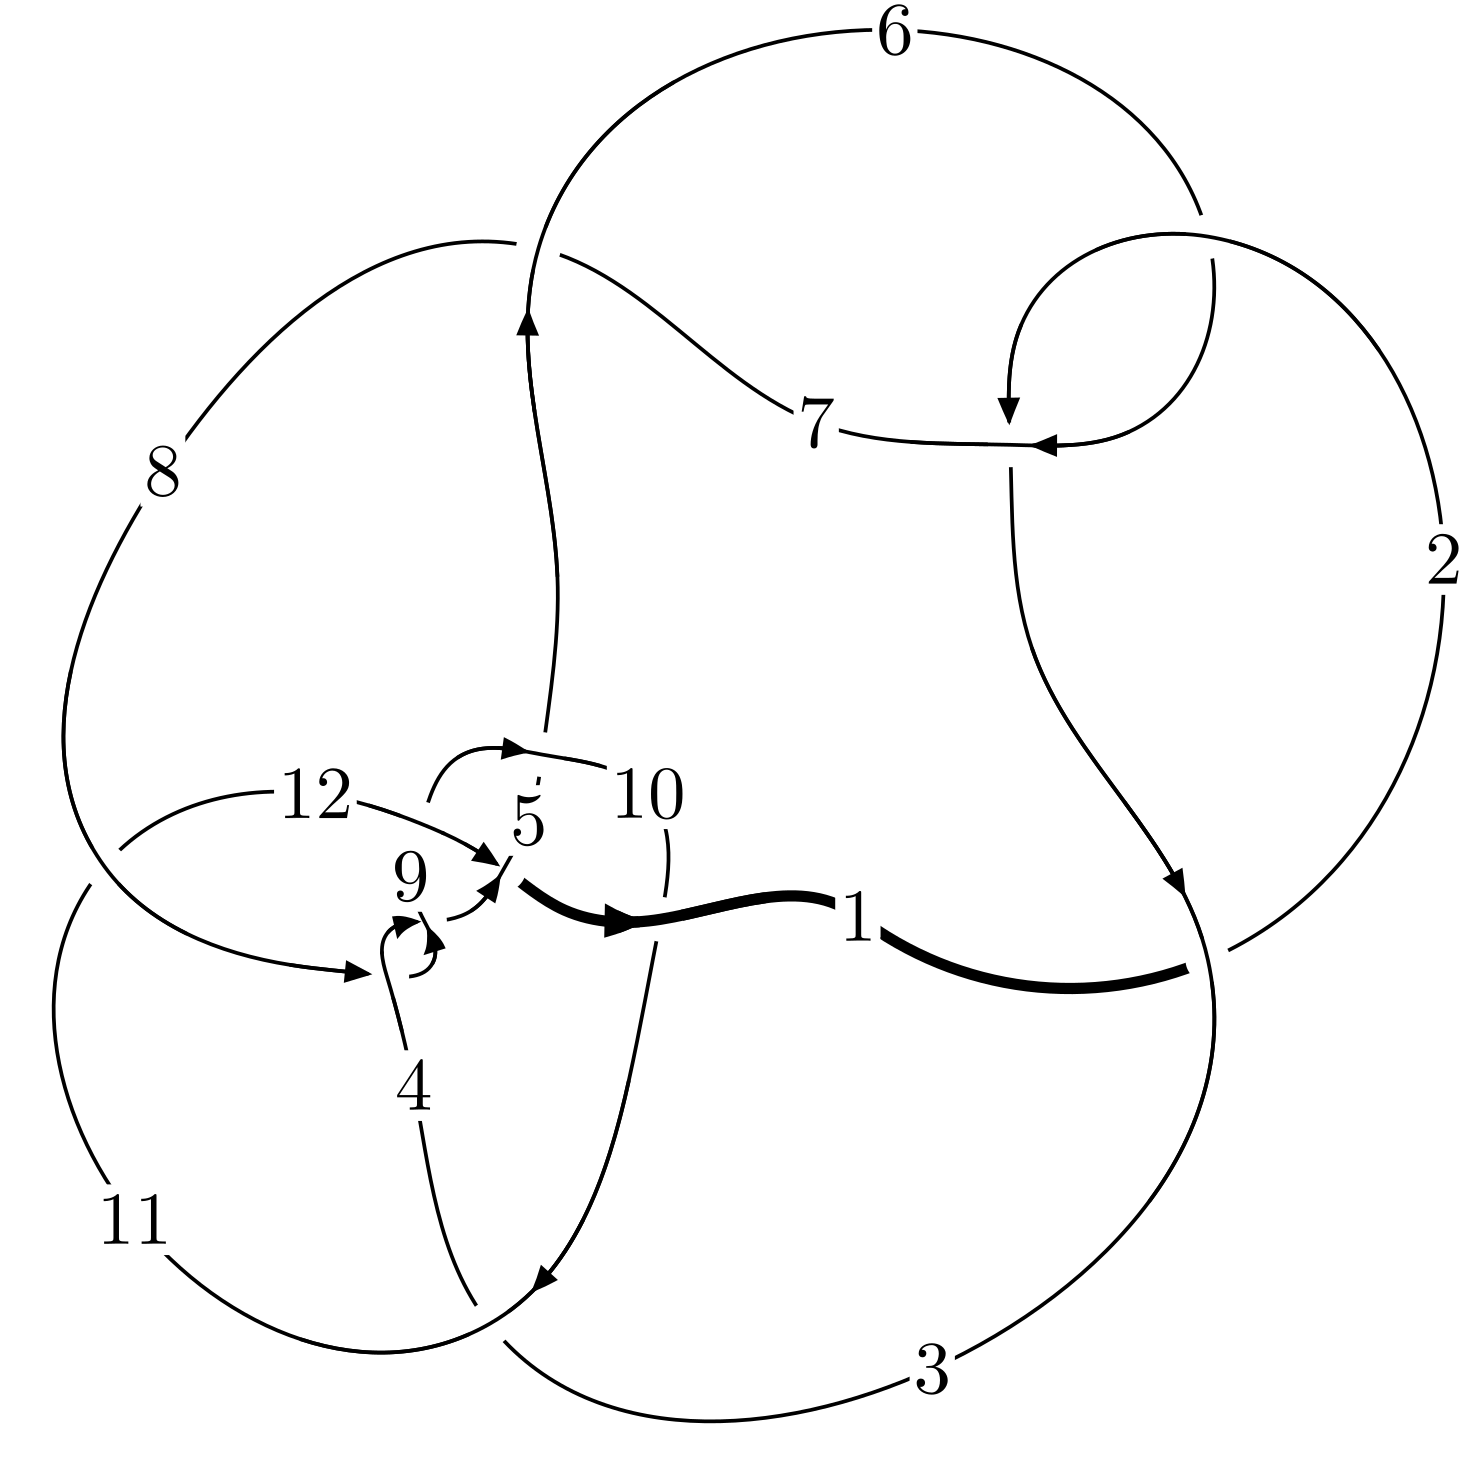
\includegraphics[width=112pt]{../../../GIT/diagram.site/Diagrams/png/1471_12a_0670.png}\\
\ \ \ A knot diagram\footnotemark}&
\allowdisplaybreaks
\textbf{Linearized knot diagam} \\
\cline{2-2}
 &
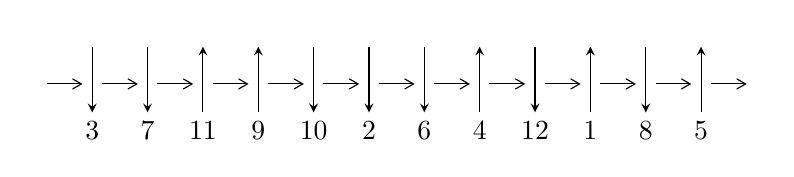
\begin{tikzpicture}[x=20pt, y=17pt]
	% nodes
	\node (C0) at (0, 0) {};
	\node (C1) at (1, 0) {};
	\node (C1U) at (1, +1) {};
	\node (C1D) at (1, -1) {3};

	\node (C2) at (2, 0) {};
	\node (C2U) at (2, +1) {};
	\node (C2D) at (2, -1) {7};

	\node (C3) at (3, 0) {};
	\node (C3U) at (3, +1) {};
	\node (C3D) at (3, -1) {11};

	\node (C4) at (4, 0) {};
	\node (C4U) at (4, +1) {};
	\node (C4D) at (4, -1) {9};

	\node (C5) at (5, 0) {};
	\node (C5U) at (5, +1) {};
	\node (C5D) at (5, -1) {10};

	\node (C6) at (6, 0) {};
	\node (C6U) at (6, +1) {};
	\node (C6D) at (6, -1) {2};

	\node (C7) at (7, 0) {};
	\node (C7U) at (7, +1) {};
	\node (C7D) at (7, -1) {6};

	\node (C8) at (8, 0) {};
	\node (C8U) at (8, +1) {};
	\node (C8D) at (8, -1) {4};

	\node (C9) at (9, 0) {};
	\node (C9U) at (9, +1) {};
	\node (C9D) at (9, -1) {12};

	\node (C10) at (10, 0) {};
	\node (C10U) at (10, +1) {};
	\node (C10D) at (10, -1) {1};

	\node (C11) at (11, 0) {};
	\node (C11U) at (11, +1) {};
	\node (C11D) at (11, -1) {8};

	\node (C12) at (12, 0) {};
	\node (C12U) at (12, +1) {};
	\node (C12D) at (12, -1) {5};
	\node (C13) at (13, 0) {};

	% arrows
	\draw[->,>={angle 60}]
	(C0) edge (C1) (C1) edge (C2) (C2) edge (C3) (C3) edge (C4) (C4) edge (C5) (C5) edge (C6) (C6) edge (C7) (C7) edge (C8) (C8) edge (C9) (C9) edge (C10) (C10) edge (C11) (C11) edge (C12) (C12) edge (C13) ;	\draw[->,>=stealth]
	(C1U) edge (C1D) (C2U) edge (C2D) (C3D) edge (C3U) (C4D) edge (C4U) (C5U) edge (C5D) (C6U) edge (C6D) (C7U) edge (C7D) (C8D) edge (C8U) (C9U) edge (C9D) (C10D) edge (C10U) (C11U) edge (C11D) (C12D) edge (C12U) ;
	\end{tikzpicture} \\
\hhline{~~} \\& 
\textbf{Solving Sequence} \\ \cline{2-2} 
 &
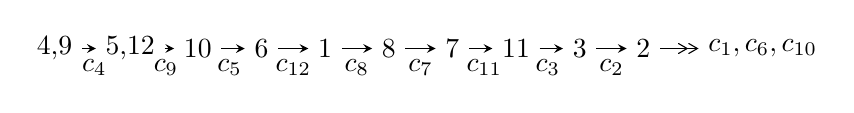
\begin{tikzpicture}[x=23pt, y=7pt]
	% node
	\node (A0) at (-1/8, 0) {4,9};
	\node (A1) at (17/16, 0) {5,12};
	\node (A2) at (17/8, 0) {10};
	\node (A3) at (25/8, 0) {6};
	\node (A4) at (33/8, 0) {1};
	\node (A5) at (41/8, 0) {8};
	\node (A6) at (49/8, 0) {7};
	\node (A7) at (57/8, 0) {11};
	\node (A8) at (65/8, 0) {3};
	\node (A9) at (73/8, 0) {2};
	\node (C1) at (1/2, -1) {$c_{4}$};
	\node (C2) at (13/8, -1) {$c_{9}$};
	\node (C3) at (21/8, -1) {$c_{5}$};
	\node (C4) at (29/8, -1) {$c_{12}$};
	\node (C5) at (37/8, -1) {$c_{8}$};
	\node (C6) at (45/8, -1) {$c_{7}$};
	\node (C7) at (53/8, -1) {$c_{11}$};
	\node (C8) at (61/8, -1) {$c_{3}$};
	\node (C9) at (69/8, -1) {$c_{2}$};
	\node (A10) at (11, 0) {$c_{1},c_{6},c_{10}$};

	% edge
	\draw[->,>=stealth]	
	(A0) edge (A1) (A1) edge (A2) (A2) edge (A3) (A3) edge (A4) (A4) edge (A5) (A5) edge (A6) (A6) edge (A7) (A7) edge (A8) (A8) edge (A9) ;
	\draw[->>,>={angle 60}]	
	(A9) edge (A10);
\end{tikzpicture} \\ 

\end{tabular} \\

\footnotetext{
The image of knot diagram is generated by the software ``\textbf{Draw programme}" developed by Andrew Bartholomew(\url{http://www.layer8.co.uk/maths/draw/index.htm\#Running-draw}), where we modified some parts for our purpose(\url{https://github.com/CATsTAILs/LinksPainter}).
}\phantom \\ \newline 
\centering \textbf{Ideals for irreducible components\footnotemark of $X_{\text{par}}$} 
 
\begin{align*}
I^u_{1}&=\langle 
-7.99478\times10^{596} u^{148}-1.64531\times10^{597} u^{147}+\cdots+3.67010\times10^{596} b-1.34656\times10^{597},\\
\phantom{I^u_{1}}&\phantom{= \langle  }-4.34564\times10^{595} u^{148}-2.62040\times10^{596} u^{147}+\cdots+3.67010\times10^{596} a-3.07089\times10^{597},\\
\phantom{I^u_{1}}&\phantom{= \langle  }u^{149}+u^{148}+\cdots-2 u-2\rangle \\
I^u_{2}&=\langle 
-1370767571 u^{29}+3000893918 u^{28}+\cdots+1426884209 b+1819309823,\\
\phantom{I^u_{2}}&\phantom{= \langle  }1090184381 u^{29}-3736521418 u^{28}+\cdots+8561305254 a-10915858938,\\
\phantom{I^u_{2}}&\phantom{= \langle  }u^{30}-2 u^{29}+\cdots+31 u^2-6\rangle \\
\\
I^v_{1}&=\langle 
a,\;b+1,\;v+1\rangle \\
\end{align*}
\raggedright * 3 irreducible components of $\dim_{\mathbb{C}}=0$, with total 180 representations.\\
\footnotetext{All coefficients of polynomials are rational numbers. But the coefficients are sometimes approximated in decimal forms when there is not enough margin.}
\newpage
\renewcommand{\arraystretch}{1}
\centering \section*{I. $I^u_{1}= \langle -7.99\times10^{596} u^{148}-1.65\times10^{597} u^{147}+\cdots+3.67\times10^{596} b-1.35\times10^{597},\;-4.35\times10^{595} u^{148}-2.62\times10^{596} u^{147}+\cdots+3.67\times10^{596} a-3.07\times10^{597},\;u^{149}+u^{148}+\cdots-2 u-2 \rangle$}
\flushleft \textbf{(i) Arc colorings}\\
\begin{tabular}{m{7pt} m{180pt} m{7pt} m{180pt} }
\flushright $a_{4}=$&$\begin{pmatrix}1\\0\end{pmatrix}$ \\
\flushright $a_{9}=$&$\begin{pmatrix}0\\u\end{pmatrix}$ \\
\flushright $a_{5}=$&$\begin{pmatrix}1\\- u^2\end{pmatrix}$ \\
\flushright $a_{12}=$&$\begin{pmatrix}0.118406 u^{148}+0.713986 u^{147}+\cdots-35.6763 u+8.36732\\2.17835 u^{148}+4.48300 u^{147}+\cdots+0.0549657 u+3.66900\end{pmatrix}$ \\
\flushright $a_{10}=$&$\begin{pmatrix}-0.713342 u^{148}-1.89845 u^{147}+\cdots-124.836 u+1.88100\\1.82739 u^{148}+3.99427 u^{147}+\cdots+9.87473 u+1.69509\end{pmatrix}$ \\
\flushright $a_{6}=$&$\begin{pmatrix}1.14943 u^{148}+3.25205 u^{147}+\cdots+93.7596 u+6.51301\\-2.07649 u^{148}-4.58001 u^{147}+\cdots-12.7746 u-2.99669\end{pmatrix}$ \\
\flushright $a_{1}=$&$\begin{pmatrix}3.19987 u^{148}+7.38147 u^{147}+\cdots-34.1933 u+13.2275\\-2.01305 u^{148}-4.61031 u^{147}+\cdots-13.2800 u-3.50305\end{pmatrix}$ \\
\flushright $a_{8}=$&$\begin{pmatrix}- u\\u\end{pmatrix}$ \\
\flushright $a_{7}=$&$\begin{pmatrix}-0.110119 u^{148}-0.935528 u^{147}+\cdots-22.2883 u-5.59236\\2.60343 u^{148}+5.86455 u^{147}+\cdots+19.0822 u+4.80160\end{pmatrix}$ \\
\flushright $a_{11}=$&$\begin{pmatrix}3.45183 u^{148}+7.86190 u^{147}+\cdots-25.2823 u+14.1678\\-1.15507 u^{148}-2.66491 u^{147}+\cdots-10.3390 u-2.13146\end{pmatrix}$ \\
\flushright $a_{3}=$&$\begin{pmatrix}1.60542 u^{148}+2.74162 u^{147}+\cdots-64.9088 u-1.39460\\0.172593 u^{148}+0.314862 u^{147}+\cdots+3.99711 u+0.132920\end{pmatrix}$ \\
\flushright $a_{2}=$&$\begin{pmatrix}4.57460 u^{148}+9.74047 u^{147}+\cdots-24.8475 u+14.0813\\-3.84852 u^{148}-8.35965 u^{147}+\cdots-12.2970 u-6.05385\end{pmatrix}$\\&\end{tabular}
\flushleft \textbf{(ii) Obstruction class $= -1$}\\~\\
\flushleft \textbf{(iii) Cusp Shapes $= 4.39778 u^{148}+8.46029 u^{147}+\cdots-64.7824 u+7.36384$}\\~\\
\newpage\renewcommand{\arraystretch}{1}
\flushleft \textbf{(iv) u-Polynomials at the component}\newline \\
\begin{tabular}{m{50pt}|m{274pt}}
Crossings & \hspace{64pt}u-Polynomials at each crossing \\
\hline $$\begin{aligned}c_{1},c_{7}\end{aligned}$$&$\begin{aligned}
&u^{149}+47 u^{148}+\cdots+102 u+1
\end{aligned}$\\
\hline $$\begin{aligned}c_{2},c_{6}\end{aligned}$$&$\begin{aligned}
&u^{149}- u^{148}+\cdots-20 u-1
\end{aligned}$\\
\hline $$\begin{aligned}c_{3}\end{aligned}$$&$\begin{aligned}
&u^{149}-27 u^{147}+\cdots-153572430 u-97971703
\end{aligned}$\\
\hline $$\begin{aligned}c_{4},c_{8}\end{aligned}$$&$\begin{aligned}
&u^{149}+u^{148}+\cdots-2 u-2
\end{aligned}$\\
\hline $$\begin{aligned}c_{5}\end{aligned}$$&$\begin{aligned}
&u^{149}+4 u^{148}+\cdots-44 u+1
\end{aligned}$\\
\hline $$\begin{aligned}c_{9}\end{aligned}$$&$\begin{aligned}
&u^{149}+3 u^{148}+\cdots-721 u+23
\end{aligned}$\\
\hline $$\begin{aligned}c_{10}\end{aligned}$$&$\begin{aligned}
&u^{149}-12 u^{148}+\cdots+84178 u-11746
\end{aligned}$\\
\hline $$\begin{aligned}c_{11}\end{aligned}$$&$\begin{aligned}
&u^{149}-4 u^{148}+\cdots-14272164 u+808439
\end{aligned}$\\
\hline $$\begin{aligned}c_{12}\end{aligned}$$&$\begin{aligned}
&u^{149}-2 u^{148}+\cdots-105006 u+72941
\end{aligned}$\\
\hline
\end{tabular}\\~\\
\newpage\renewcommand{\arraystretch}{1}
\flushleft \textbf{(v) Riley Polynomials at the component}\newline \\
\begin{tabular}{m{50pt}|m{274pt}}
Crossings & \hspace{64pt}Riley Polynomials at each crossing \\
\hline $$\begin{aligned}c_{1},c_{7}\end{aligned}$$&$\begin{aligned}
&y^{149}+117 y^{148}+\cdots-5398 y-1
\end{aligned}$\\
\hline $$\begin{aligned}c_{2},c_{6}\end{aligned}$$&$\begin{aligned}
&y^{149}-47 y^{148}+\cdots+102 y-1
\end{aligned}$\\
\hline $$\begin{aligned}c_{3}\end{aligned}$$&$\begin{aligned}
&y^{149}-54 y^{148}+\cdots+618907160688127504 y-9598454588720209
\end{aligned}$\\
\hline $$\begin{aligned}c_{4},c_{8}\end{aligned}$$&$\begin{aligned}
&y^{149}-115 y^{148}+\cdots-1060 y-4
\end{aligned}$\\
\hline $$\begin{aligned}c_{5}\end{aligned}$$&$\begin{aligned}
&y^{149}-12 y^{148}+\cdots+134 y-1
\end{aligned}$\\
\hline $$\begin{aligned}c_{9}\end{aligned}$$&$\begin{aligned}
&y^{149}+21 y^{148}+\cdots+46639 y-529
\end{aligned}$\\
\hline $$\begin{aligned}c_{10}\end{aligned}$$&$\begin{aligned}
&y^{149}-42 y^{148}+\cdots-5433937780 y-137968516
\end{aligned}$\\
\hline $$\begin{aligned}c_{11}\end{aligned}$$&$\begin{aligned}
&y^{149}+34 y^{148}+\cdots+2349436602660 y-653573616721
\end{aligned}$\\
\hline $$\begin{aligned}c_{12}\end{aligned}$$&$\begin{aligned}
&y^{149}-36 y^{148}+\cdots+321679207278 y-5320389481
\end{aligned}$\\
\hline
\end{tabular}\\~\\
\newpage\flushleft \textbf{(vi) Complex Volumes and Cusp Shapes}
$$\begin{array}{c|c|c}  
\text{Solutions to }I^u_{1}& \I (\text{vol} + \sqrt{-1}CS) & \text{Cusp shape}\\
 \hline 
\begin{aligned}
u &= -0.997927 + 0.108985 I \\
a &= \phantom{-}0.342836 + 0.881654 I \\
b &= -1.08945 - 1.35487 I\end{aligned}
 & \phantom{-}2.61641 - 5.27304 I & \phantom{-0.000000 } 0 \\ \hline\begin{aligned}
u &= -0.997927 - 0.108985 I \\
a &= \phantom{-}0.342836 - 0.881654 I \\
b &= -1.08945 + 1.35487 I\end{aligned}
 & \phantom{-}2.61641 + 5.27304 I & \phantom{-0.000000 } 0 \\ \hline\begin{aligned}
u &= \phantom{-}0.906099 + 0.405833 I \\
a &= \phantom{-}0.269225 - 0.454312 I \\
b &= \phantom{-}0.565957 + 1.151150 I\end{aligned}
 & \phantom{-}1.54507 + 1.61217 I & \phantom{-0.000000 } 0 \\ \hline\begin{aligned}
u &= \phantom{-}0.906099 - 0.405833 I \\
a &= \phantom{-}0.269225 + 0.454312 I \\
b &= \phantom{-}0.565957 - 1.151150 I\end{aligned}
 & \phantom{-}1.54507 - 1.61217 I & \phantom{-0.000000 } 0 \\ \hline\begin{aligned}
u &= -1.03753\phantom{ +0.000000I} \\
a &= \phantom{-}1.36639\phantom{ +0.000000I} \\
b &= \phantom{-}0.0654382\phantom{ +0.000000I}\end{aligned}
 & -1.53008\phantom{ +0.000000I} & \phantom{-0.000000 } 0 \\ \hline\begin{aligned}
u &= \phantom{-}1.044210 + 0.037573 I \\
a &= -0.110451 + 0.886146 I \\
b &= \phantom{-}0.82417 - 1.45728 I\end{aligned}
 & \phantom{-}3.25938 - 0.03179 I & \phantom{-0.000000 } 0 \\ \hline\begin{aligned}
u &= \phantom{-}1.044210 - 0.037573 I \\
a &= -0.110451 - 0.886146 I \\
b &= \phantom{-}0.82417 + 1.45728 I\end{aligned}
 & \phantom{-}3.25938 + 0.03179 I & \phantom{-0.000000 } 0 \\ \hline\begin{aligned}
u &= -1.040440 + 0.109520 I \\
a &= \phantom{-}1.23894 + 0.91114 I \\
b &= -0.235026 - 1.199110 I\end{aligned}
 & \phantom{-}1.86508 - 5.73127 I & \phantom{-0.000000 } 0 \\ \hline\begin{aligned}
u &= -1.040440 - 0.109520 I \\
a &= \phantom{-}1.23894 - 0.91114 I \\
b &= -0.235026 + 1.199110 I\end{aligned}
 & \phantom{-}1.86508 + 5.73127 I & \phantom{-0.000000 } 0 \\ \hline\begin{aligned}
u &= \phantom{-}0.902583 + 0.304485 I \\
a &= \phantom{-}0.184569 - 0.327460 I \\
b &= \phantom{-}0.47442 + 1.48814 I\end{aligned}
 & \phantom{-}1.51854 + 1.59281 I & \phantom{-0.000000 } 0\\
 \hline 
 \end{array}$$\newpage$$\begin{array}{c|c|c}  
\text{Solutions to }I^u_{1}& \I (\text{vol} + \sqrt{-1}CS) & \text{Cusp shape}\\
 \hline 
\begin{aligned}
u &= \phantom{-}0.902583 - 0.304485 I \\
a &= \phantom{-}0.184569 + 0.327460 I \\
b &= \phantom{-}0.47442 - 1.48814 I\end{aligned}
 & \phantom{-}1.51854 - 1.59281 I & \phantom{-0.000000 } 0 \\ \hline\begin{aligned}
u &= \phantom{-}1.028050 + 0.210019 I \\
a &= -1.00999 + 1.40491 I \\
b &= \phantom{-}0.53800 - 1.60291 I\end{aligned}
 & \phantom{-}1.95414 + 1.08684 I & \phantom{-0.000000 } 0 \\ \hline\begin{aligned}
u &= \phantom{-}1.028050 - 0.210019 I \\
a &= -1.00999 - 1.40491 I \\
b &= \phantom{-}0.53800 + 1.60291 I\end{aligned}
 & \phantom{-}1.95414 - 1.08684 I & \phantom{-0.000000 } 0 \\ \hline\begin{aligned}
u &= -1.013410 + 0.378410 I \\
a &= -0.190732 - 0.276665 I \\
b &= \phantom{-}0.45155 + 1.63437 I\end{aligned}
 & -1.58390 - 5.31842 I & \phantom{-0.000000 } 0 \\ \hline\begin{aligned}
u &= -1.013410 - 0.378410 I \\
a &= -0.190732 + 0.276665 I \\
b &= \phantom{-}0.45155 - 1.63437 I\end{aligned}
 & -1.58390 + 5.31842 I & \phantom{-0.000000 } 0 \\ \hline\begin{aligned}
u &= -0.678394 + 0.611928 I \\
a &= -0.113690 - 0.113990 I \\
b &= \phantom{-}0.126935 + 0.634408 I\end{aligned}
 & -1.82938 + 0.95182 I & \phantom{-0.000000 } 0 \\ \hline\begin{aligned}
u &= -0.678394 - 0.611928 I \\
a &= -0.113690 + 0.113990 I \\
b &= \phantom{-}0.126935 - 0.634408 I\end{aligned}
 & -1.82938 - 0.95182 I & \phantom{-0.000000 } 0 \\ \hline\begin{aligned}
u &= \phantom{-}0.411545 + 0.810144 I \\
a &= -1.226940 + 0.398074 I \\
b &= \phantom{-}0.557464 + 0.684261 I\end{aligned}
 & \phantom{-}1.66303 - 5.32531 I & \phantom{-0.000000 } 0 \\ \hline\begin{aligned}
u &= \phantom{-}0.411545 - 0.810144 I \\
a &= -1.226940 - 0.398074 I \\
b &= \phantom{-}0.557464 - 0.684261 I\end{aligned}
 & \phantom{-}1.66303 + 5.32531 I & \phantom{-0.000000 } 0 \\ \hline\begin{aligned}
u &= -0.380989 + 0.823004 I \\
a &= \phantom{-}1.193010 + 0.378164 I \\
b &= -0.473274 + 0.663865 I\end{aligned}
 & \phantom{-}1.92473 - 0.27110 I & \phantom{-0.000000 } 0\\
 \hline 
 \end{array}$$\newpage$$\begin{array}{c|c|c}  
\text{Solutions to }I^u_{1}& \I (\text{vol} + \sqrt{-1}CS) & \text{Cusp shape}\\
 \hline 
\begin{aligned}
u &= -0.380989 - 0.823004 I \\
a &= \phantom{-}1.193010 - 0.378164 I \\
b &= -0.473274 - 0.663865 I\end{aligned}
 & \phantom{-}1.92473 + 0.27110 I & \phantom{-0.000000 } 0 \\ \hline\begin{aligned}
u &= -0.148141 + 1.088790 I \\
a &= \phantom{-}0.708479 - 0.269615 I \\
b &= \phantom{-}0.125862 + 0.354257 I\end{aligned}
 & \phantom{-}5.70505 + 4.15041 I & \phantom{-0.000000 } 0 \\ \hline\begin{aligned}
u &= -0.148141 - 1.088790 I \\
a &= \phantom{-}0.708479 + 0.269615 I \\
b &= \phantom{-}0.125862 - 0.354257 I\end{aligned}
 & \phantom{-}5.70505 - 4.15041 I & \phantom{-0.000000 } 0 \\ \hline\begin{aligned}
u &= \phantom{-}1.103690 + 0.037743 I \\
a &= -0.801369 + 0.434320 I \\
b &= -0.844166 - 1.086500 I\end{aligned}
 & \phantom{-}3.35672 + 1.40100 I & \phantom{-0.000000 } 0 \\ \hline\begin{aligned}
u &= \phantom{-}1.103690 - 0.037743 I \\
a &= -0.801369 - 0.434320 I \\
b &= -0.844166 + 1.086500 I\end{aligned}
 & \phantom{-}3.35672 - 1.40100 I & \phantom{-0.000000 } 0 \\ \hline\begin{aligned}
u &= \phantom{-}1.056740 + 0.344471 I \\
a &= -0.54907 + 1.57577 I \\
b &= \phantom{-}0.70639 - 1.83078 I\end{aligned}
 & -0.92505 + 5.62393 I & \phantom{-0.000000 } 0 \\ \hline\begin{aligned}
u &= \phantom{-}1.056740 - 0.344471 I \\
a &= -0.54907 - 1.57577 I \\
b &= \phantom{-}0.70639 + 1.83078 I\end{aligned}
 & -0.92505 - 5.62393 I & \phantom{-0.000000 } 0 \\ \hline\begin{aligned}
u &= \phantom{-}0.145293 + 1.111540 I \\
a &= -0.671311 - 0.344539 I \\
b &= -0.133325 + 0.308302 I\end{aligned}
 & \phantom{-}6.18629 + 2.02105 I & \phantom{-0.000000 } 0 \\ \hline\begin{aligned}
u &= \phantom{-}0.145293 - 1.111540 I \\
a &= -0.671311 + 0.344539 I \\
b &= -0.133325 - 0.308302 I\end{aligned}
 & \phantom{-}6.18629 - 2.02105 I & \phantom{-0.000000 } 0 \\ \hline\begin{aligned}
u &= \phantom{-}1.109490 + 0.277234 I \\
a &= \phantom{-}0.166987 - 0.353004 I \\
b &= -0.89151 + 2.34886 I\end{aligned}
 & \phantom{-}6.46485 + 4.62859 I & \phantom{-0.000000 } 0\\
 \hline 
 \end{array}$$\newpage$$\begin{array}{c|c|c}  
\text{Solutions to }I^u_{1}& \I (\text{vol} + \sqrt{-1}CS) & \text{Cusp shape}\\
 \hline 
\begin{aligned}
u &= \phantom{-}1.109490 - 0.277234 I \\
a &= \phantom{-}0.166987 + 0.353004 I \\
b &= -0.89151 - 2.34886 I\end{aligned}
 & \phantom{-}6.46485 - 4.62859 I & \phantom{-0.000000 } 0 \\ \hline\begin{aligned}
u &= -0.169120 + 1.139590 I \\
a &= \phantom{-}0.561589 - 0.856111 I \\
b &= \phantom{-}0.0796304 - 0.0369593 I\end{aligned}
 & \phantom{-}3.2097 - 13.9267 I & \phantom{-0.000000 } 0 \\ \hline\begin{aligned}
u &= -0.169120 - 1.139590 I \\
a &= \phantom{-}0.561589 + 0.856111 I \\
b &= \phantom{-}0.0796304 + 0.0369593 I\end{aligned}
 & \phantom{-}3.2097 + 13.9267 I & \phantom{-0.000000 } 0 \\ \hline\begin{aligned}
u &= \phantom{-}0.170592 + 1.143440 I \\
a &= -0.566518 - 0.816153 I \\
b &= -0.0918103 - 0.0056737 I\end{aligned}
 & \phantom{-}4.21112 + 7.80500 I & \phantom{-0.000000 } 0 \\ \hline\begin{aligned}
u &= \phantom{-}0.170592 - 1.143440 I \\
a &= -0.566518 + 0.816153 I \\
b &= -0.0918103 + 0.0056737 I\end{aligned}
 & \phantom{-}4.21112 - 7.80500 I & \phantom{-0.000000 } 0 \\ \hline\begin{aligned}
u &= -0.191524 + 1.144560 I \\
a &= \phantom{-}0.416254 - 0.791031 I \\
b &= -0.0115438 + 0.0464869 I\end{aligned}
 & -3.41519 - 7.81442 I & \phantom{-0.000000 } 0 \\ \hline\begin{aligned}
u &= -0.191524 - 1.144560 I \\
a &= \phantom{-}0.416254 + 0.791031 I \\
b &= -0.0115438 - 0.0464869 I\end{aligned}
 & -3.41519 + 7.81442 I & \phantom{-0.000000 } 0 \\ \hline\begin{aligned}
u &= -1.127820 + 0.301148 I \\
a &= -0.191953 - 0.360112 I \\
b &= \phantom{-}1.00539 + 2.20383 I\end{aligned}
 & \phantom{-}5.59100 - 10.86960 I & \phantom{-0.000000 } 0 \\ \hline\begin{aligned}
u &= -1.127820 - 0.301148 I \\
a &= -0.191953 + 0.360112 I \\
b &= \phantom{-}1.00539 - 2.20383 I\end{aligned}
 & \phantom{-}5.59100 + 10.86960 I & \phantom{-0.000000 } 0 \\ \hline\begin{aligned}
u &= \phantom{-}1.082960 + 0.447710 I \\
a &= -0.24765 + 1.57941 I \\
b &= \phantom{-}0.78257 - 1.92036 I\end{aligned}
 & \phantom{-}3.77855 + 10.04870 I & \phantom{-0.000000 } 0\\
 \hline 
 \end{array}$$\newpage$$\begin{array}{c|c|c}  
\text{Solutions to }I^u_{1}& \I (\text{vol} + \sqrt{-1}CS) & \text{Cusp shape}\\
 \hline 
\begin{aligned}
u &= \phantom{-}1.082960 - 0.447710 I \\
a &= -0.24765 - 1.57941 I \\
b &= \phantom{-}0.78257 + 1.92036 I\end{aligned}
 & \phantom{-}3.77855 - 10.04870 I & \phantom{-0.000000 } 0 \\ \hline\begin{aligned}
u &= -0.507320 + 0.650379 I \\
a &= -0.524205 - 0.737183 I \\
b &= -0.649181 + 0.518377 I\end{aligned}
 & -3.12048 + 1.18009 I & \phantom{-0.000000 } 0 \\ \hline\begin{aligned}
u &= -0.507320 - 0.650379 I \\
a &= -0.524205 + 0.737183 I \\
b &= -0.649181 - 0.518377 I\end{aligned}
 & -3.12048 - 1.18009 I & \phantom{-0.000000 } 0 \\ \hline\begin{aligned}
u &= \phantom{-}0.174954 + 1.166670 I \\
a &= -0.450111 - 0.641115 I \\
b &= -0.0389245 + 0.1320640 I\end{aligned}
 & \phantom{-}0.70784 + 4.41763 I & \phantom{-0.000000 } 0 \\ \hline\begin{aligned}
u &= \phantom{-}0.174954 - 1.166670 I \\
a &= -0.450111 + 0.641115 I \\
b &= -0.0389245 - 0.1320640 I\end{aligned}
 & \phantom{-}0.70784 - 4.41763 I & \phantom{-0.000000 } 0 \\ \hline\begin{aligned}
u &= \phantom{-}0.441941 + 0.688681 I \\
a &= -1.244180 + 0.491058 I \\
b &= \phantom{-}0.766708 + 0.442072 I\end{aligned}
 & -2.78657 - 1.63532 I & \phantom{-0.000000 } 0 \\ \hline\begin{aligned}
u &= \phantom{-}0.441941 - 0.688681 I \\
a &= -1.244180 - 0.491058 I \\
b &= \phantom{-}0.766708 - 0.442072 I\end{aligned}
 & -2.78657 + 1.63532 I & \phantom{-0.000000 } 0 \\ \hline\begin{aligned}
u &= -0.118484 + 0.802160 I \\
a &= \phantom{-}0.658374 + 0.514246 I \\
b &= -0.135012 + 0.329816 I\end{aligned}
 & -1.15927 + 1.43856 I & \phantom{-0.000000 } 0 \\ \hline\begin{aligned}
u &= -0.118484 - 0.802160 I \\
a &= \phantom{-}0.658374 - 0.514246 I \\
b &= -0.135012 - 0.329816 I\end{aligned}
 & -1.15927 - 1.43856 I & \phantom{-0.000000 } 0 \\ \hline\begin{aligned}
u &= -1.181650 + 0.176133 I \\
a &= \phantom{-}0.617217 + 1.067780 I \\
b &= -0.15319 - 2.14924 I\end{aligned}
 & \phantom{-}2.11194 - 5.30881 I & \phantom{-0.000000 } 0\\
 \hline 
 \end{array}$$\newpage$$\begin{array}{c|c|c}  
\text{Solutions to }I^u_{1}& \I (\text{vol} + \sqrt{-1}CS) & \text{Cusp shape}\\
 \hline 
\begin{aligned}
u &= -1.181650 - 0.176133 I \\
a &= \phantom{-}0.617217 - 1.067780 I \\
b &= -0.15319 + 2.14924 I\end{aligned}
 & \phantom{-}2.11194 + 5.30881 I & \phantom{-0.000000 } 0 \\ \hline\begin{aligned}
u &= \phantom{-}1.193300 + 0.084273 I \\
a &= \phantom{-}0.86821 + 1.31202 I \\
b &= -0.31384 - 2.13053 I\end{aligned}
 & \phantom{-}2.34030 + 4.44114 I & \phantom{-0.000000 } 0 \\ \hline\begin{aligned}
u &= \phantom{-}1.193300 - 0.084273 I \\
a &= \phantom{-}0.86821 - 1.31202 I \\
b &= -0.31384 + 2.13053 I\end{aligned}
 & \phantom{-}2.34030 - 4.44114 I & \phantom{-0.000000 } 0 \\ \hline\begin{aligned}
u &= \phantom{-}0.559855 + 0.572285 I \\
a &= -1.222220 + 0.512666 I \\
b &= \phantom{-}1.102970 + 0.206290 I\end{aligned}
 & \phantom{-}0.80054 + 2.00529 I & \phantom{-0.000000 } 0 \\ \hline\begin{aligned}
u &= \phantom{-}0.559855 - 0.572285 I \\
a &= -1.222220 - 0.512666 I \\
b &= \phantom{-}1.102970 - 0.206290 I\end{aligned}
 & \phantom{-}0.80054 - 2.00529 I & \phantom{-0.000000 } 0 \\ \hline\begin{aligned}
u &= \phantom{-}1.196670 + 0.109755 I \\
a &= \phantom{-}1.29187 + 1.46649 I \\
b &= -0.83459 - 2.42562 I\end{aligned}
 & \phantom{-}8.10417 + 9.47321 I & \phantom{-0.000000 } 0 \\ \hline\begin{aligned}
u &= \phantom{-}1.196670 - 0.109755 I \\
a &= \phantom{-}1.29187 - 1.46649 I \\
b &= -0.83459 + 2.42562 I\end{aligned}
 & \phantom{-}8.10417 - 9.47321 I & \phantom{-0.000000 } 0 \\ \hline\begin{aligned}
u &= -1.116450 + 0.450429 I \\
a &= \phantom{-}0.22416 + 1.49263 I \\
b &= -0.75745 - 1.94000 I\end{aligned}
 & \phantom{-}4.25390 - 4.49520 I & \phantom{-0.000000 } 0 \\ \hline\begin{aligned}
u &= -1.116450 - 0.450429 I \\
a &= \phantom{-}0.22416 - 1.49263 I \\
b &= -0.75745 + 1.94000 I\end{aligned}
 & \phantom{-}4.25390 + 4.49520 I & \phantom{-0.000000 } 0 \\ \hline\begin{aligned}
u &= -1.203530 + 0.109989 I \\
a &= -1.32160 + 1.34085 I \\
b &= \phantom{-}0.90485 - 2.26970 I\end{aligned}
 & \phantom{-}8.87316 - 3.63122 I & \phantom{-0.000000 } 0\\
 \hline 
 \end{array}$$\newpage$$\begin{array}{c|c|c}  
\text{Solutions to }I^u_{1}& \I (\text{vol} + \sqrt{-1}CS) & \text{Cusp shape}\\
 \hline 
\begin{aligned}
u &= -1.203530 - 0.109989 I \\
a &= -1.32160 - 1.34085 I \\
b &= \phantom{-}0.90485 + 2.26970 I\end{aligned}
 & \phantom{-}8.87316 + 3.63122 I & \phantom{-0.000000 } 0 \\ \hline\begin{aligned}
u &= -1.004700 + 0.672684 I \\
a &= -0.305368 - 0.565052 I \\
b &= -0.256201 + 0.933577 I\end{aligned}
 & -0.90910 - 6.47182 I & \phantom{-0.000000 } 0 \\ \hline\begin{aligned}
u &= -1.004700 - 0.672684 I \\
a &= -0.305368 + 0.565052 I \\
b &= -0.256201 - 0.933577 I\end{aligned}
 & -0.90910 + 6.47182 I & \phantom{-0.000000 } 0 \\ \hline\begin{aligned}
u &= \phantom{-}1.212300 + 0.032402 I \\
a &= \phantom{-}0.377505 - 0.653265 I \\
b &= \phantom{-}0.311166 + 1.221160 I\end{aligned}
 & \phantom{-}3.18267 + 0.49662 I & \phantom{-0.000000 } 0 \\ \hline\begin{aligned}
u &= \phantom{-}1.212300 - 0.032402 I \\
a &= \phantom{-}0.377505 + 0.653265 I \\
b &= \phantom{-}0.311166 - 1.221160 I\end{aligned}
 & \phantom{-}3.18267 - 0.49662 I & \phantom{-0.000000 } 0 \\ \hline\begin{aligned}
u &= \phantom{-}1.226990 + 0.039571 I \\
a &= -0.361508 + 0.786450 I \\
b &= -0.83365 - 2.52866 I\end{aligned}
 & \phantom{-}9.27492 + 2.42864 I & \phantom{-0.000000 } 0 \\ \hline\begin{aligned}
u &= \phantom{-}1.226990 - 0.039571 I \\
a &= -0.361508 - 0.786450 I \\
b &= -0.83365 + 2.52866 I\end{aligned}
 & \phantom{-}9.27492 - 2.42864 I & \phantom{-0.000000 } 0 \\ \hline\begin{aligned}
u &= -1.228560 + 0.075364 I \\
a &= -0.987214 + 0.906544 I \\
b &= \phantom{-}0.55372 - 1.59986 I\end{aligned}
 & \phantom{-}5.51292 - 1.98562 I & \phantom{-0.000000 } 0 \\ \hline\begin{aligned}
u &= -1.228560 - 0.075364 I \\
a &= -0.987214 - 0.906544 I \\
b &= \phantom{-}0.55372 + 1.59986 I\end{aligned}
 & \phantom{-}5.51292 + 1.98562 I & \phantom{-0.000000 } 0 \\ \hline\begin{aligned}
u &= -0.576590 + 0.507170 I \\
a &= \phantom{-}1.179340 + 0.491640 I \\
b &= -1.132470 + 0.046145 I\end{aligned}
 & \phantom{-}0.87292 + 3.33988 I & \phantom{-0.000000 } 0\\
 \hline 
 \end{array}$$\newpage$$\begin{array}{c|c|c}  
\text{Solutions to }I^u_{1}& \I (\text{vol} + \sqrt{-1}CS) & \text{Cusp shape}\\
 \hline 
\begin{aligned}
u &= -0.576590 - 0.507170 I \\
a &= \phantom{-}1.179340 - 0.491640 I \\
b &= -1.132470 - 0.046145 I\end{aligned}
 & \phantom{-}0.87292 - 3.33988 I & \phantom{-0.000000 } 0 \\ \hline\begin{aligned}
u &= -1.196990 + 0.303365 I \\
a &= \phantom{-}0.500611 + 1.233240 I \\
b &= -0.69194 - 2.05863 I\end{aligned}
 & \phantom{-}1.91368 - 4.83833 I & \phantom{-0.000000 } 0 \\ \hline\begin{aligned}
u &= -1.196990 - 0.303365 I \\
a &= \phantom{-}0.500611 - 1.233240 I \\
b &= -0.69194 + 2.05863 I\end{aligned}
 & \phantom{-}1.91368 + 4.83833 I & \phantom{-0.000000 } 0 \\ \hline\begin{aligned}
u &= -0.178626 + 1.227670 I \\
a &= \phantom{-}0.288378 - 0.542263 I \\
b &= -0.021204 + 0.202786 I\end{aligned}
 & -2.55049 - 0.20359 I & \phantom{-0.000000 } 0 \\ \hline\begin{aligned}
u &= -0.178626 - 1.227670 I \\
a &= \phantom{-}0.288378 + 0.542263 I \\
b &= -0.021204 - 0.202786 I\end{aligned}
 & -2.55049 + 0.20359 I & \phantom{-0.000000 } 0 \\ \hline\begin{aligned}
u &= -1.240650 + 0.054760 I \\
a &= \phantom{-}0.362471 + 0.843791 I \\
b &= \phantom{-}0.70178 - 2.61256 I\end{aligned}
 & \phantom{-}8.83349 - 8.53833 I & \phantom{-0.000000 } 0 \\ \hline\begin{aligned}
u &= -1.240650 - 0.054760 I \\
a &= \phantom{-}0.362471 - 0.843791 I \\
b &= \phantom{-}0.70178 + 2.61256 I\end{aligned}
 & \phantom{-}8.83349 + 8.53833 I & \phantom{-0.000000 } 0 \\ \hline\begin{aligned}
u &= -0.005854 + 0.708081 I \\
a &= -0.13905 + 1.67581 I \\
b &= -0.014455 + 0.174742 I\end{aligned}
 & -1.01217 + 2.55939 I & \phantom{-0.000000 } 0 \\ \hline\begin{aligned}
u &= -0.005854 - 0.708081 I \\
a &= -0.13905 - 1.67581 I \\
b &= -0.014455 - 0.174742 I\end{aligned}
 & -1.01217 - 2.55939 I & \phantom{-0.000000 } 0 \\ \hline\begin{aligned}
u &= -0.698550 + 0.110191 I \\
a &= \phantom{-}0.548182 + 0.333374 I \\
b &= -0.919508 - 0.688389 I\end{aligned}
 & -1.95646 - 0.51661 I & \phantom{-0.000000 } 0\\
 \hline 
 \end{array}$$\newpage$$\begin{array}{c|c|c}  
\text{Solutions to }I^u_{1}& \I (\text{vol} + \sqrt{-1}CS) & \text{Cusp shape}\\
 \hline 
\begin{aligned}
u &= -0.698550 - 0.110191 I \\
a &= \phantom{-}0.548182 - 0.333374 I \\
b &= -0.919508 + 0.688389 I\end{aligned}
 & -1.95646 + 0.51661 I & \phantom{-0.000000 } 0 \\ \hline\begin{aligned}
u &= -1.299100 + 0.113301 I \\
a &= -1.309760 + 0.378513 I \\
b &= \phantom{-}1.20596 - 0.91158 I\end{aligned}
 & \phantom{-}8.76797 - 0.64485 I & \phantom{-0.000000 } 0 \\ \hline\begin{aligned}
u &= -1.299100 - 0.113301 I \\
a &= -1.309760 - 0.378513 I \\
b &= \phantom{-}1.20596 + 0.91158 I\end{aligned}
 & \phantom{-}8.76797 + 0.64485 I & \phantom{-0.000000 } 0 \\ \hline\begin{aligned}
u &= \phantom{-}1.281160 + 0.292066 I \\
a &= -0.540452 + 1.164070 I \\
b &= \phantom{-}1.13995 - 2.32706 I\end{aligned}
 & -0.22552 + 5.20204 I & \phantom{-0.000000 } 0 \\ \hline\begin{aligned}
u &= \phantom{-}1.281160 - 0.292066 I \\
a &= -0.540452 - 1.164070 I \\
b &= \phantom{-}1.13995 + 2.32706 I\end{aligned}
 & -0.22552 - 5.20204 I & \phantom{-0.000000 } 0 \\ \hline\begin{aligned}
u &= -1.293040 + 0.250167 I \\
a &= \phantom{-}0.498078 + 1.191740 I \\
b &= -0.85502 - 2.71580 I\end{aligned}
 & \phantom{-}4.64814 - 3.64822 I & \phantom{-0.000000 } 0 \\ \hline\begin{aligned}
u &= -1.293040 - 0.250167 I \\
a &= \phantom{-}0.498078 - 1.191740 I \\
b &= -0.85502 + 2.71580 I\end{aligned}
 & \phantom{-}4.64814 + 3.64822 I & \phantom{-0.000000 } 0 \\ \hline\begin{aligned}
u &= \phantom{-}1.298360 + 0.262420 I \\
a &= -0.509838 + 1.201720 I \\
b &= \phantom{-}0.98641 - 2.70994 I\end{aligned}
 & \phantom{-}4.30570 + 9.22114 I & \phantom{-0.000000 } 0 \\ \hline\begin{aligned}
u &= \phantom{-}1.298360 - 0.262420 I \\
a &= -0.509838 - 1.201720 I \\
b &= \phantom{-}0.98641 + 2.70994 I\end{aligned}
 & \phantom{-}4.30570 - 9.22114 I & \phantom{-0.000000 } 0 \\ \hline\begin{aligned}
u &= \phantom{-}1.294890 + 0.298366 I \\
a &= -0.593820 + 1.053360 I \\
b &= \phantom{-}1.34923 - 1.89030 I\end{aligned}
 & \phantom{-}3.04546 + 1.07755 I & \phantom{-0.000000 } 0\\
 \hline 
 \end{array}$$\newpage$$\begin{array}{c|c|c}  
\text{Solutions to }I^u_{1}& \I (\text{vol} + \sqrt{-1}CS) & \text{Cusp shape}\\
 \hline 
\begin{aligned}
u &= \phantom{-}1.294890 - 0.298366 I \\
a &= -0.593820 - 1.053360 I \\
b &= \phantom{-}1.34923 + 1.89030 I\end{aligned}
 & \phantom{-}3.04546 - 1.07755 I & \phantom{-0.000000 } 0 \\ \hline\begin{aligned}
u &= \phantom{-}1.324670 + 0.118649 I \\
a &= \phantom{-}1.300120 + 0.239979 I \\
b &= -1.26577 - 0.69203 I\end{aligned}
 & \phantom{-}7.92836 - 5.05927 I & \phantom{-0.000000 } 0 \\ \hline\begin{aligned}
u &= \phantom{-}1.324670 - 0.118649 I \\
a &= \phantom{-}1.300120 - 0.239979 I \\
b &= -1.26577 + 0.69203 I\end{aligned}
 & \phantom{-}7.92836 + 5.05927 I & \phantom{-0.000000 } 0 \\ \hline\begin{aligned}
u &= -0.168792 + 0.644253 I \\
a &= \phantom{-}1.075160 + 0.846995 I \\
b &= -0.303616 + 0.146890 I\end{aligned}
 & -1.26238 + 1.26752 I & \phantom{-0.000000 } 0 \\ \hline\begin{aligned}
u &= -0.168792 - 0.644253 I \\
a &= \phantom{-}1.075160 - 0.846995 I \\
b &= -0.303616 - 0.146890 I\end{aligned}
 & -1.26238 - 1.26752 I & \phantom{-0.000000 } 0 \\ \hline\begin{aligned}
u &= \phantom{-}1.33728\phantom{ +0.000000I} \\
a &= \phantom{-}0.884739\phantom{ +0.000000I} \\
b &= -0.562692\phantom{ +0.000000I}\end{aligned}
 & \phantom{-}3.14559\phantom{ +0.000000I} & \phantom{-0.000000 } 0 \\ \hline\begin{aligned}
u &= -0.225743 + 0.605662 I \\
a &= -0.85345 - 1.22257 I \\
b &= -0.871486 + 0.326644 I\end{aligned}
 & \phantom{-}2.94982 + 7.40247 I & \phantom{-0.000000 } 0. - 6.37798 I \\ \hline\begin{aligned}
u &= -0.225743 - 0.605662 I \\
a &= -0.85345 + 1.22257 I \\
b &= -0.871486 - 0.326644 I\end{aligned}
 & \phantom{-}2.94982 - 7.40247 I & \phantom{-0.000000 -}0. + 6.37798 I \\ \hline\begin{aligned}
u &= -0.024150 + 0.637120 I \\
a &= -0.76910 + 1.73292 I \\
b &= -0.0225561 + 0.0154055 I\end{aligned}
 & -4.27900 - 1.74395 I & -13.30081 + 4.30618 I \\ \hline\begin{aligned}
u &= -0.024150 - 0.637120 I \\
a &= -0.76910 - 1.73292 I \\
b &= -0.0225561 - 0.0154055 I\end{aligned}
 & -4.27900 + 1.74395 I & -13.30081 - 4.30618 I\\
 \hline 
 \end{array}$$\newpage$$\begin{array}{c|c|c}  
\text{Solutions to }I^u_{1}& \I (\text{vol} + \sqrt{-1}CS) & \text{Cusp shape}\\
 \hline 
\begin{aligned}
u &= -1.335710 + 0.305614 I \\
a &= \phantom{-}0.542047 + 0.916983 I \\
b &= -1.20357 - 1.59570 I\end{aligned}
 & \phantom{-}3.15814 - 6.05638 I & \phantom{-0.000000 } 0 \\ \hline\begin{aligned}
u &= -1.335710 - 0.305614 I \\
a &= \phantom{-}0.542047 - 0.916983 I \\
b &= -1.20357 + 1.59570 I\end{aligned}
 & \phantom{-}3.15814 + 6.05638 I & \phantom{-0.000000 } 0 \\ \hline\begin{aligned}
u &= -1.37438\phantom{ +0.000000I} \\
a &= -0.140023\phantom{ +0.000000I} \\
b &= -1.04115\phantom{ +0.000000I}\end{aligned}
 & \phantom{-}3.78742\phantom{ +0.000000I} & \phantom{-0.000000 } 0 \\ \hline\begin{aligned}
u &= \phantom{-}1.374070 + 0.094273 I \\
a &= \phantom{-}0.064446 - 0.305779 I \\
b &= \phantom{-}1.135960 + 0.807885 I\end{aligned}
 & \phantom{-}8.10829 + 2.97693 I & \phantom{-0.000000 } 0 \\ \hline\begin{aligned}
u &= \phantom{-}1.374070 - 0.094273 I \\
a &= \phantom{-}0.064446 + 0.305779 I \\
b &= \phantom{-}1.135960 - 0.807885 I\end{aligned}
 & \phantom{-}8.10829 - 2.97693 I & \phantom{-0.000000 } 0 \\ \hline\begin{aligned}
u &= -1.387360 + 0.076160 I \\
a &= -0.046875 - 0.247195 I \\
b &= -1.218360 + 0.665416 I\end{aligned}
 & \phantom{-}8.06310 + 2.74688 I & \phantom{-0.000000 } 0 \\ \hline\begin{aligned}
u &= -1.387360 - 0.076160 I \\
a &= -0.046875 + 0.247195 I \\
b &= -1.218360 - 0.665416 I\end{aligned}
 & \phantom{-}8.06310 - 2.74688 I & \phantom{-0.000000 } 0 \\ \hline\begin{aligned}
u &= \phantom{-}0.234686 + 0.541606 I \\
a &= \phantom{-}1.03150 - 1.12299 I \\
b &= \phantom{-}0.896775 + 0.385966 I\end{aligned}
 & \phantom{-}3.98355 - 1.42403 I & \phantom{-0.000000 -}0. + 1.79463 I \\ \hline\begin{aligned}
u &= \phantom{-}0.234686 - 0.541606 I \\
a &= \phantom{-}1.03150 + 1.12299 I \\
b &= \phantom{-}0.896775 - 0.385966 I\end{aligned}
 & \phantom{-}3.98355 + 1.42403 I & \phantom{-0.000000 } 0. - 1.79463 I \\ \hline\begin{aligned}
u &= -1.36420 + 0.45250 I \\
a &= \phantom{-}0.161610 + 0.880893 I \\
b &= -0.59823 - 1.58574 I\end{aligned}
 & \phantom{-}2.88325 - 6.18656 I & \phantom{-0.000000 } 0\\
 \hline 
 \end{array}$$\newpage$$\begin{array}{c|c|c}  
\text{Solutions to }I^u_{1}& \I (\text{vol} + \sqrt{-1}CS) & \text{Cusp shape}\\
 \hline 
\begin{aligned}
u &= -1.36420 - 0.45250 I \\
a &= \phantom{-}0.161610 - 0.880893 I \\
b &= -0.59823 + 1.58574 I\end{aligned}
 & \phantom{-}2.88325 + 6.18656 I & \phantom{-0.000000 } 0 \\ \hline\begin{aligned}
u &= -0.097025 + 0.541005 I \\
a &= -1.18908 + 2.16565 I \\
b &= -0.074791 - 0.242803 I\end{aligned}
 & -0.00951 - 6.14995 I & -5.15912 + 9.56291 I \\ \hline\begin{aligned}
u &= -0.097025 - 0.541005 I \\
a &= -1.18908 - 2.16565 I \\
b &= -0.074791 + 0.242803 I\end{aligned}
 & -0.00951 + 6.14995 I & -5.15912 - 9.56291 I \\ \hline\begin{aligned}
u &= \phantom{-}1.37299 + 0.46766 I \\
a &= \phantom{-}0.249032 - 0.815727 I \\
b &= -0.10539 + 1.89819 I\end{aligned}
 & \phantom{-}10.47990 + 1.18464 I & \phantom{-0.000000 } 0 \\ \hline\begin{aligned}
u &= \phantom{-}1.37299 - 0.46766 I \\
a &= \phantom{-}0.249032 + 0.815727 I \\
b &= -0.10539 - 1.89819 I\end{aligned}
 & \phantom{-}10.47990 - 1.18464 I & \phantom{-0.000000 } 0 \\ \hline\begin{aligned}
u &= -1.38714 + 0.47525 I \\
a &= -0.270723 - 0.849451 I \\
b &= \phantom{-}0.21800 + 1.95630 I\end{aligned}
 & \phantom{-}11.00770 - 7.48541 I & \phantom{-0.000000 } 0 \\ \hline\begin{aligned}
u &= -1.38714 - 0.47525 I \\
a &= -0.270723 + 0.849451 I \\
b &= \phantom{-}0.21800 - 1.95630 I\end{aligned}
 & \phantom{-}11.00770 + 7.48541 I & \phantom{-0.000000 } 0 \\ \hline\begin{aligned}
u &= -1.37607 + 0.58086 I \\
a &= -0.155294 + 0.832237 I \\
b &= -0.14543 - 1.72501 I\end{aligned}
 & \phantom{-}9.60663 - 10.29480 I & \phantom{-0.000000 } 0 \\ \hline\begin{aligned}
u &= -1.37607 - 0.58086 I \\
a &= -0.155294 - 0.832237 I \\
b &= -0.14543 + 1.72501 I\end{aligned}
 & \phantom{-}9.60663 + 10.29480 I & \phantom{-0.000000 } 0 \\ \hline\begin{aligned}
u &= -1.41561 + 0.50043 I \\
a &= -0.411580 - 0.926096 I \\
b &= \phantom{-}0.69454 + 1.93625 I\end{aligned}
 & \phantom{-}5.66364 - 10.19030 I & \phantom{-0.000000 } 0\\
 \hline 
 \end{array}$$\newpage$$\begin{array}{c|c|c}  
\text{Solutions to }I^u_{1}& \I (\text{vol} + \sqrt{-1}CS) & \text{Cusp shape}\\
 \hline 
\begin{aligned}
u &= -1.41561 - 0.50043 I \\
a &= -0.411580 + 0.926096 I \\
b &= \phantom{-}0.69454 - 1.93625 I\end{aligned}
 & \phantom{-}5.66364 + 10.19030 I & \phantom{-0.000000 } 0 \\ \hline\begin{aligned}
u &= \phantom{-}1.41066 + 0.51448 I \\
a &= \phantom{-}0.433834 - 0.845199 I \\
b &= -0.63455 + 1.70913 I\end{aligned}
 & \phantom{-}2.35588 + 6.14144 I & \phantom{-0.000000 } 0 \\ \hline\begin{aligned}
u &= \phantom{-}1.41066 - 0.51448 I \\
a &= \phantom{-}0.433834 + 0.845199 I \\
b &= -0.63455 - 1.70913 I\end{aligned}
 & \phantom{-}2.35588 - 6.14144 I & \phantom{-0.000000 } 0 \\ \hline\begin{aligned}
u &= \phantom{-}1.42266 + 0.50171 I \\
a &= \phantom{-}0.473417 - 0.965723 I \\
b &= -0.89654 + 1.93561 I\end{aligned}
 & \phantom{-}1.60032 + 13.57150 I & \phantom{-0.000000 } 0 \\ \hline\begin{aligned}
u &= \phantom{-}1.42266 - 0.50171 I \\
a &= \phantom{-}0.473417 + 0.965723 I \\
b &= -0.89654 - 1.93561 I\end{aligned}
 & \phantom{-}1.60032 - 13.57150 I & \phantom{-0.000000 } 0 \\ \hline\begin{aligned}
u &= -1.42480 + 0.49787 I \\
a &= -0.426359 - 1.032130 I \\
b &= \phantom{-}0.89552 + 2.15822 I\end{aligned}
 & \phantom{-}9.2092 - 13.5493 I & \phantom{-0.000000 } 0 \\ \hline\begin{aligned}
u &= -1.42480 - 0.49787 I \\
a &= -0.426359 + 1.032130 I \\
b &= \phantom{-}0.89552 - 2.15822 I\end{aligned}
 & \phantom{-}9.2092 + 13.5493 I & \phantom{-0.000000 } 0 \\ \hline\begin{aligned}
u &= \phantom{-}0.079356 + 0.483845 I \\
a &= \phantom{-}1.49364 + 2.17335 I \\
b &= -0.023160 - 0.323983 I\end{aligned}
 & \phantom{-}0.400754 + 0.769646 I & -3.62764 - 4.22124 I \\ \hline\begin{aligned}
u &= \phantom{-}0.079356 - 0.483845 I \\
a &= \phantom{-}1.49364 - 2.17335 I \\
b &= -0.023160 + 0.323983 I\end{aligned}
 & \phantom{-}0.400754 - 0.769646 I & -3.62764 + 4.22124 I \\ \hline\begin{aligned}
u &= \phantom{-}1.42541 + 0.49897 I \\
a &= \phantom{-}0.444191 - 1.046960 I \\
b &= -0.95958 + 2.16163 I\end{aligned}
 & \phantom{-}8.2043 + 19.6713 I & \phantom{-0.000000 } 0\\
 \hline 
 \end{array}$$\newpage$$\begin{array}{c|c|c}  
\text{Solutions to }I^u_{1}& \I (\text{vol} + \sqrt{-1}CS) & \text{Cusp shape}\\
 \hline 
\begin{aligned}
u &= \phantom{-}1.42541 - 0.49897 I \\
a &= \phantom{-}0.444191 + 1.046960 I \\
b &= -0.95958 - 2.16163 I\end{aligned}
 & \phantom{-}8.2043 - 19.6713 I & \phantom{-0.000000 } 0 \\ \hline\begin{aligned}
u &= \phantom{-}1.39525 + 0.58208 I \\
a &= \phantom{-}0.149798 + 0.780263 I \\
b &= \phantom{-}0.10433 - 1.64635 I\end{aligned}
 & \phantom{-}10.17640 + 4.23781 I & \phantom{-0.000000 } 0 \\ \hline\begin{aligned}
u &= \phantom{-}1.39525 - 0.58208 I \\
a &= \phantom{-}0.149798 - 0.780263 I \\
b &= \phantom{-}0.10433 + 1.64635 I\end{aligned}
 & \phantom{-}10.17640 - 4.23781 I & \phantom{-0.000000 } 0 \\ \hline\begin{aligned}
u &= \phantom{-}1.51992 + 0.49926 I \\
a &= -0.079425 + 0.555517 I \\
b &= \phantom{-}0.320286 - 1.115130 I\end{aligned}
 & \phantom{-}5.20990 + 2.59443 I & \phantom{-0.000000 } 0 \\ \hline\begin{aligned}
u &= \phantom{-}1.51992 - 0.49926 I \\
a &= -0.079425 - 0.555517 I \\
b &= \phantom{-}0.320286 + 1.115130 I\end{aligned}
 & \phantom{-}5.20990 - 2.59443 I & \phantom{-0.000000 } 0 \\ \hline\begin{aligned}
u &= \phantom{-}0.256326 + 0.097023 I \\
a &= \phantom{-}1.15434 + 1.45578 I \\
b &= \phantom{-}0.837599 + 0.492157 I\end{aligned}
 & \phantom{-}1.35101 + 1.14697 I & \phantom{-}4.21689 - 0.23530 I \\ \hline\begin{aligned}
u &= \phantom{-}0.256326 - 0.097023 I \\
a &= \phantom{-}1.15434 - 1.45578 I \\
b &= \phantom{-}0.837599 - 0.492157 I\end{aligned}
 & \phantom{-}1.35101 - 1.14697 I & \phantom{-}4.21689 + 0.23530 I \\ \hline\begin{aligned}
u &= \phantom{-}1.59558 + 0.74938 I \\
a &= \phantom{-}0.132239 + 0.277814 I \\
b &= -0.262690 - 0.665385 I\end{aligned}
 & \phantom{-}7.92798 - 0.71672 I & \phantom{-0.000000 } 0 \\ \hline\begin{aligned}
u &= \phantom{-}1.59558 - 0.74938 I \\
a &= \phantom{-}0.132239 - 0.277814 I \\
b &= -0.262690 + 0.665385 I\end{aligned}
 & \phantom{-}7.92798 + 0.71672 I & \phantom{-0.000000 } 0 \\ \hline\begin{aligned}
u &= -1.56554 + 0.82526 I \\
a &= -0.165697 + 0.215774 I \\
b &= \phantom{-}0.376825 - 0.530305 I\end{aligned}
 & \phantom{-}6.78955 + 6.87071 I & \phantom{-0.000000 } 0\\
 \hline 
 \end{array}$$\newpage$$\begin{array}{c|c|c}  
\text{Solutions to }I^u_{1}& \I (\text{vol} + \sqrt{-1}CS) & \text{Cusp shape}\\
 \hline 
\begin{aligned}
u &= -1.56554 - 0.82526 I \\
a &= -0.165697 - 0.215774 I \\
b &= \phantom{-}0.376825 + 0.530305 I\end{aligned}
 & \phantom{-}6.78955 - 6.87071 I & \phantom{-0.000000 } 0 \\ \hline\begin{aligned}
u &= -0.050337 + 0.143727 I \\
a &= \phantom{-}6.05261 - 4.40226 I \\
b &= \phantom{-}0.895601 + 0.771524 I\end{aligned}
 & \phantom{-}5.51740 + 2.45186 I & \phantom{-}1.48976 - 2.21266 I \\ \hline\begin{aligned}
u &= -0.050337 - 0.143727 I \\
a &= \phantom{-}6.05261 + 4.40226 I \\
b &= \phantom{-}0.895601 - 0.771524 I\end{aligned}
 & \phantom{-}5.51740 - 2.45186 I & \phantom{-}1.48976 + 2.21266 I \\ \hline\begin{aligned}
u &= \phantom{-}0.088004 + 0.112374 I \\
a &= -5.42303 - 6.59172 I \\
b &= -0.859983 + 0.833552 I\end{aligned}
 & \phantom{-}4.87849 - 8.36632 I & \phantom{-}0.05497 + 7.74602 I \\ \hline\begin{aligned}
u &= \phantom{-}0.088004 - 0.112374 I \\
a &= -5.42303 + 6.59172 I \\
b &= -0.859983 - 0.833552 I\end{aligned}
 & \phantom{-}4.87849 + 8.36632 I & \phantom{-}0.05497 - 7.74602 I \\ \hline\begin{aligned}
u &= -1.85064 + 0.34572 I \\
a &= \phantom{-}0.195358 + 0.196008 I \\
b &= -0.417037 - 0.389154 I\end{aligned}
 & \phantom{-}0.691007 - 0.095500 I & \phantom{-0.000000 } 0 \\ \hline\begin{aligned}
u &= -1.85064 - 0.34572 I \\
a &= \phantom{-}0.195358 - 0.196008 I \\
b &= -0.417037 + 0.389154 I\end{aligned}
 & \phantom{-}0.691007 + 0.095500 I & \phantom{-0.000000 } 0 \\ \hline\begin{aligned}
u &= -0.0329582 + 0.0764814 I \\
a &= \phantom{-}10.97440 - 2.70410 I \\
b &= -0.627852 - 0.639342 I\end{aligned}
 & -1.12585 + 3.89050 I & -4.12840 - 7.88335 I \\ \hline\begin{aligned}
u &= -0.0329582 - 0.0764814 I \\
a &= \phantom{-}10.97440 + 2.70410 I \\
b &= -0.627852 + 0.639342 I\end{aligned}
 & -1.12585 - 3.89050 I & -4.12840 + 7.88335 I\\
 \hline 
 \end{array}$$\newpage\newpage\renewcommand{\arraystretch}{1}
\centering \section*{II. $I^u_{2}= \langle -1.37\times10^{9} u^{29}+3.00\times10^{9} u^{28}+\cdots+1.43\times10^{9} b+1.82\times10^{9},\;1.09\times10^{9} u^{29}-3.74\times10^{9} u^{28}+\cdots+8.56\times10^{9} a-1.09\times10^{10},\;u^{30}-2 u^{29}+\cdots+31 u^2-6 \rangle$}
\flushleft \textbf{(i) Arc colorings}\\
\begin{tabular}{m{7pt} m{180pt} m{7pt} m{180pt} }
\flushright $a_{4}=$&$\begin{pmatrix}1\\0\end{pmatrix}$ \\
\flushright $a_{9}=$&$\begin{pmatrix}0\\u\end{pmatrix}$ \\
\flushright $a_{5}=$&$\begin{pmatrix}1\\- u^2\end{pmatrix}$ \\
\flushright $a_{12}=$&$\begin{pmatrix}-0.127339 u^{29}+0.436443 u^{28}+\cdots-4.56981 u+1.27502\\0.960672 u^{29}-2.10311 u^{28}+\cdots+4.40314 u-1.27502\end{pmatrix}$ \\
\flushright $a_{10}=$&$\begin{pmatrix}2.07198 u^{29}-2.79558 u^{28}+\cdots+5.20462 u+5.29242\\-2.74171 u^{29}+3.42548 u^{28}+\cdots-12.7928 u-8.27471\end{pmatrix}$ \\
\flushright $a_{6}=$&$\begin{pmatrix}-0.227533 u^{29}-1.39875 u^{28}+\cdots+2.05216 u-1.11252\\0.788279 u^{29}+1.94488 u^{28}+\cdots-0.0942501 u+8.90838\end{pmatrix}$ \\
\flushright $a_{1}=$&$\begin{pmatrix}0.376233 u^{29}-0.679520 u^{28}+\cdots-0.930698 u+1.09059\\0.492373 u^{29}-0.980821 u^{28}+\cdots+1.38171 u-0.622106\end{pmatrix}$ \\
\flushright $a_{8}=$&$\begin{pmatrix}- u\\u\end{pmatrix}$ \\
\flushright $a_{7}=$&$\begin{pmatrix}0.373633 u^{29}-1.55557 u^{28}+\cdots-2.41411 u+5.11324\\0.364926 u^{29}+1.57166 u^{28}+\cdots-3.04829 u-1.99902\end{pmatrix}$ \\
\flushright $a_{11}=$&$\begin{pmatrix}0.872661 u^{29}-1.56356 u^{28}+\cdots+0.430194 u+1.27502\\-0.0393281 u^{29}-0.103110 u^{28}+\cdots-0.596861 u-1.27502\end{pmatrix}$ \\
\flushright $a_{3}=$&$\begin{pmatrix}-0.0399878 u^{29}+0.736908 u^{28}+\cdots-0.839954 u+1.75607\\-0.457062 u^{29}-1.24587 u^{28}+\cdots-1.03510 u-9.17756\end{pmatrix}$ \\
\flushright $a_{2}=$&$\begin{pmatrix}-1.20801 u^{29}+1.48368 u^{28}+\cdots-18.4085 u-6.68528\\0.252875 u^{29}-1.22381 u^{28}+\cdots+12.8874 u+2.35677\end{pmatrix}$\\&\end{tabular}
\flushleft \textbf{(ii) Obstruction class $= 1$}\\~\\
\flushleft \textbf{(iii) Cusp Shapes $= -\frac{1857898437}{1426884209} u^{29}+\frac{1101274625}{1426884209} u^{28}+\cdots-\frac{2246147754}{1426884209} u+\frac{2439848022}{1426884209}$}\\~\\
\newpage\renewcommand{\arraystretch}{1}
\flushleft \textbf{(iv) u-Polynomials at the component}\newline \\
\begin{tabular}{m{50pt}|m{274pt}}
Crossings & \hspace{64pt}u-Polynomials at each crossing \\
\hline $$\begin{aligned}c_{1}\end{aligned}$$&$\begin{aligned}
&u^{30}-11 u^{29}+\cdots-24 u+1
\end{aligned}$\\
\hline $$\begin{aligned}c_{2}\end{aligned}$$&$\begin{aligned}
&u^{30}+u^{29}+\cdots-2 u+1
\end{aligned}$\\
\hline $$\begin{aligned}c_{3}\end{aligned}$$&$\begin{aligned}
&u^{30}+u^{28}+\cdots-4 u-1
\end{aligned}$\\
\hline $$\begin{aligned}c_{4}\end{aligned}$$&$\begin{aligned}
&u^{30}-2 u^{29}+\cdots+31 u^2-6
\end{aligned}$\\
\hline $$\begin{aligned}c_{5}\end{aligned}$$&$\begin{aligned}
&u^{30}-2 u^{29}+\cdots+2 u^2-1
\end{aligned}$\\
\hline $$\begin{aligned}c_{6}\end{aligned}$$&$\begin{aligned}
&u^{30}- u^{29}+\cdots+2 u+1
\end{aligned}$\\
\hline $$\begin{aligned}c_{7}\end{aligned}$$&$\begin{aligned}
&u^{30}+11 u^{29}+\cdots+24 u+1
\end{aligned}$\\
\hline $$\begin{aligned}c_{8}\end{aligned}$$&$\begin{aligned}
&u^{30}+2 u^{29}+\cdots+31 u^2-6
\end{aligned}$\\
\hline $$\begin{aligned}c_{9}\end{aligned}$$&$\begin{aligned}
&u^{30}-15 u^{29}+\cdots- u+1
\end{aligned}$\\
\hline $$\begin{aligned}c_{10}\end{aligned}$$&$\begin{aligned}
&u^{30}+15 u^{29}+\cdots+84 u+6
\end{aligned}$\\
\hline $$\begin{aligned}c_{11}\end{aligned}$$&$\begin{aligned}
&u^{30}-2 u^{29}+\cdots+2 u+1
\end{aligned}$\\
\hline $$\begin{aligned}c_{12}\end{aligned}$$&$\begin{aligned}
&u^{30}-2 u^{28}+\cdots-2 u-1
\end{aligned}$\\
\hline
\end{tabular}\\~\\
\newpage\renewcommand{\arraystretch}{1}
\flushleft \textbf{(v) Riley Polynomials at the component}\newline \\
\begin{tabular}{m{50pt}|m{274pt}}
Crossings & \hspace{64pt}Riley Polynomials at each crossing \\
\hline $$\begin{aligned}c_{1},c_{7}\end{aligned}$$&$\begin{aligned}
&y^{30}+21 y^{29}+\cdots-188 y+1
\end{aligned}$\\
\hline $$\begin{aligned}c_{2},c_{6}\end{aligned}$$&$\begin{aligned}
&y^{30}-11 y^{29}+\cdots-24 y+1
\end{aligned}$\\
\hline $$\begin{aligned}c_{3}\end{aligned}$$&$\begin{aligned}
&y^{30}+2 y^{29}+\cdots-10 y+1
\end{aligned}$\\
\hline $$\begin{aligned}c_{4},c_{8}\end{aligned}$$&$\begin{aligned}
&y^{30}-28 y^{29}+\cdots-372 y+36
\end{aligned}$\\
\hline $$\begin{aligned}c_{5}\end{aligned}$$&$\begin{aligned}
&y^{30}-12 y^{29}+\cdots-4 y+1
\end{aligned}$\\
\hline $$\begin{aligned}c_{9}\end{aligned}$$&$\begin{aligned}
&y^{30}+9 y^{29}+\cdots-33 y+1
\end{aligned}$\\
\hline $$\begin{aligned}c_{10}\end{aligned}$$&$\begin{aligned}
&y^{30}+9 y^{29}+\cdots+348 y+36
\end{aligned}$\\
\hline $$\begin{aligned}c_{11}\end{aligned}$$&$\begin{aligned}
&y^{30}+10 y^{29}+\cdots-14 y+1
\end{aligned}$\\
\hline $$\begin{aligned}c_{12}\end{aligned}$$&$\begin{aligned}
&y^{30}-4 y^{29}+\cdots-12 y+1
\end{aligned}$\\
\hline
\end{tabular}\\~\\
\newpage\flushleft \textbf{(vi) Complex Volumes and Cusp Shapes}
$$\begin{array}{c|c|c}  
\text{Solutions to }I^u_{2}& \I (\text{vol} + \sqrt{-1}CS) & \text{Cusp shape}\\
 \hline 
\begin{aligned}
u &= \phantom{-}0.104625 + 0.923256 I \\
a &= \phantom{-}0.265809 + 0.752869 I \\
b &= -0.391165 - 0.185290 I\end{aligned}
 & -2.70916 - 0.36347 I & -5.68779 + 2.55332 I \\ \hline\begin{aligned}
u &= \phantom{-}0.104625 - 0.923256 I \\
a &= \phantom{-}0.265809 - 0.752869 I \\
b &= -0.391165 + 0.185290 I\end{aligned}
 & -2.70916 + 0.36347 I & -5.68779 - 2.55332 I \\ \hline\begin{aligned}
u &= \phantom{-}0.925210 + 0.632705 I \\
a &= -0.306492 + 0.692770 I \\
b &= -0.287678 - 1.045560 I\end{aligned}
 & -1.04921 + 6.74209 I & -6.9717 - 17.6770 I \\ \hline\begin{aligned}
u &= \phantom{-}0.925210 - 0.632705 I \\
a &= -0.306492 - 0.692770 I \\
b &= -0.287678 + 1.045560 I\end{aligned}
 & -1.04921 - 6.74209 I & -6.9717 + 17.6770 I \\ \hline\begin{aligned}
u &= \phantom{-}0.441570 + 0.740792 I \\
a &= -0.983711 + 0.177248 I \\
b &= \phantom{-}0.339960 + 0.247380 I\end{aligned}
 & -1.58554 - 2.14623 I & -3.91271 + 8.26189 I \\ \hline\begin{aligned}
u &= \phantom{-}0.441570 - 0.740792 I \\
a &= -0.983711 - 0.177248 I \\
b &= \phantom{-}0.339960 - 0.247380 I\end{aligned}
 & -1.58554 + 2.14623 I & -3.91271 - 8.26189 I \\ \hline\begin{aligned}
u &= -1.112230 + 0.248377 I \\
a &= -0.294821 + 0.999761 I \\
b &= \phantom{-}0.16233 - 2.50771 I\end{aligned}
 & \phantom{-}7.23517 - 3.77455 I & \phantom{-}4.79539 + 3.05652 I \\ \hline\begin{aligned}
u &= -1.112230 - 0.248377 I \\
a &= -0.294821 - 0.999761 I \\
b &= \phantom{-}0.16233 + 2.50771 I\end{aligned}
 & \phantom{-}7.23517 + 3.77455 I & \phantom{-}4.79539 - 3.05652 I \\ \hline\begin{aligned}
u &= \phantom{-}1.124510 + 0.246615 I \\
a &= \phantom{-}0.306505 + 1.165960 I \\
b &= -0.10708 - 2.62249 I\end{aligned}
 & \phantom{-}6.63030 + 9.75976 I & \phantom{-}3.08859 - 8.59497 I \\ \hline\begin{aligned}
u &= \phantom{-}1.124510 - 0.246615 I \\
a &= \phantom{-}0.306505 - 1.165960 I \\
b &= -0.10708 + 2.62249 I\end{aligned}
 & \phantom{-}6.63030 - 9.75976 I & \phantom{-}3.08859 + 8.59497 I\\
 \hline 
 \end{array}$$\newpage$$\begin{array}{c|c|c}  
\text{Solutions to }I^u_{2}& \I (\text{vol} + \sqrt{-1}CS) & \text{Cusp shape}\\
 \hline 
\begin{aligned}
u &= -0.778457 + 0.328988 I \\
a &= \phantom{-}0.398578 + 0.589993 I \\
b &= \phantom{-}1.12365 - 1.22530 I\end{aligned}
 & \phantom{-}1.51678 - 1.96575 I & -2.8548 + 16.4537 I \\ \hline\begin{aligned}
u &= -0.778457 - 0.328988 I \\
a &= \phantom{-}0.398578 - 0.589993 I \\
b &= \phantom{-}1.12365 + 1.22530 I\end{aligned}
 & \phantom{-}1.51678 + 1.96575 I & -2.8548 - 16.4537 I \\ \hline\begin{aligned}
u &= \phantom{-}1.182520 + 0.271936 I \\
a &= -0.272567 + 1.344390 I \\
b &= \phantom{-}0.54579 - 2.45540 I\end{aligned}
 & \phantom{-}0.73006 + 5.74512 I & -2.34178 - 9.28764 I \\ \hline\begin{aligned}
u &= \phantom{-}1.182520 - 0.271936 I \\
a &= -0.272567 - 1.344390 I \\
b &= \phantom{-}0.54579 + 2.45540 I\end{aligned}
 & \phantom{-}0.73006 - 5.74512 I & -2.34178 + 9.28764 I \\ \hline\begin{aligned}
u &= \phantom{-}1.237030 + 0.243287 I \\
a &= -0.70204 + 1.46894 I \\
b &= \phantom{-}1.17190 - 2.39427 I\end{aligned}
 & \phantom{-}3.45679 + 2.11535 I & \phantom{-}1.86259 - 3.59666 I \\ \hline\begin{aligned}
u &= \phantom{-}1.237030 - 0.243287 I \\
a &= -0.70204 - 1.46894 I \\
b &= \phantom{-}1.17190 + 2.39427 I\end{aligned}
 & \phantom{-}3.45679 - 2.11535 I & \phantom{-}1.86259 + 3.59666 I \\ \hline\begin{aligned}
u &= -1.259130 + 0.250394 I \\
a &= \phantom{-}0.79304 + 1.33981 I \\
b &= -1.24553 - 2.17631 I\end{aligned}
 & \phantom{-}3.46355 - 7.24797 I & \phantom{-}1.94305 + 9.64259 I \\ \hline\begin{aligned}
u &= -1.259130 - 0.250394 I \\
a &= \phantom{-}0.79304 - 1.33981 I \\
b &= -1.24553 + 2.17631 I\end{aligned}
 & \phantom{-}3.46355 + 7.24797 I & \phantom{-}1.94305 - 9.64259 I \\ \hline\begin{aligned}
u &= -1.248090 + 0.349855 I \\
a &= \phantom{-}0.546044 + 0.996300 I \\
b &= -0.69469 - 1.77284 I\end{aligned}
 & \phantom{-}1.21720 - 3.87858 I & -2.76696 + 1.67621 I \\ \hline\begin{aligned}
u &= -1.248090 - 0.349855 I \\
a &= \phantom{-}0.546044 - 0.996300 I \\
b &= -0.69469 + 1.77284 I\end{aligned}
 & \phantom{-}1.21720 + 3.87858 I & -2.76696 - 1.67621 I\\
 \hline 
 \end{array}$$\newpage$$\begin{array}{c|c|c}  
\text{Solutions to }I^u_{2}& \I (\text{vol} + \sqrt{-1}CS) & \text{Cusp shape}\\
 \hline 
\begin{aligned}
u &= -1.30305\phantom{ +0.000000I} \\
a &= -0.317222\phantom{ +0.000000I} \\
b &= -0.782350\phantom{ +0.000000I}\end{aligned}
 & \phantom{-}4.70302\phantom{ +0.000000I} & \phantom{-}9.03370\phantom{ +0.000000I} \\ \hline\begin{aligned}
u &= -1.338130 + 0.381633 I \\
a &= -0.311838 - 0.253564 I \\
b &= \phantom{-}0.144327 - 0.317309 I\end{aligned}
 & \phantom{-}7.27001 + 0.65287 I & \phantom{-}1.72726 - 0.56653 I \\ \hline\begin{aligned}
u &= -1.338130 - 0.381633 I \\
a &= -0.311838 + 0.253564 I \\
b &= \phantom{-}0.144327 + 0.317309 I\end{aligned}
 & \phantom{-}7.27001 - 0.65287 I & \phantom{-}1.72726 + 0.56653 I \\ \hline\begin{aligned}
u &= \phantom{-}1.298550 + 0.502261 I \\
a &= \phantom{-}0.214115 - 0.362845 I \\
b &= -0.239125 - 0.159015 I\end{aligned}
 & \phantom{-}6.34080 - 6.56667 I & -0.38431 + 3.74652 I \\ \hline\begin{aligned}
u &= \phantom{-}1.298550 - 0.502261 I \\
a &= \phantom{-}0.214115 + 0.362845 I \\
b &= -0.239125 + 0.159015 I\end{aligned}
 & \phantom{-}6.34080 + 6.56667 I & -0.38431 - 3.74652 I \\ \hline\begin{aligned}
u &= \phantom{-}0.434303 + 0.407723 I \\
a &= -2.20800 + 0.15427 I \\
b &= \phantom{-}0.724963 + 0.483771 I\end{aligned}
 & \phantom{-}0.610816 + 0.510651 I & -4.13449 - 1.23404 I \\ \hline\begin{aligned}
u &= \phantom{-}0.434303 - 0.407723 I \\
a &= -2.20800 - 0.15427 I \\
b &= \phantom{-}0.724963 - 0.483771 I\end{aligned}
 & \phantom{-}0.610816 - 0.510651 I & -4.13449 + 1.23404 I \\ \hline\begin{aligned}
u &= -0.389560 + 0.331187 I \\
a &= \phantom{-}2.65743 + 0.42275 I \\
b &= -0.875054 + 0.419543 I\end{aligned}
 & \phantom{-}0.28706 + 4.74128 I & -5.56195 - 4.45765 I \\ \hline\begin{aligned}
u &= -0.389560 - 0.331187 I \\
a &= \phantom{-}2.65743 - 0.42275 I \\
b &= -0.875054 - 0.419543 I\end{aligned}
 & \phantom{-}0.28706 - 4.74128 I & -5.56195 + 4.45765 I \\ \hline\begin{aligned}
u &= \phantom{-}2.05761\phantom{ +0.000000I} \\
a &= \phantom{-}0.113135\phantom{ +0.000000I} \\
b &= \phantom{-}0.0371552\phantom{ +0.000000I}\end{aligned}
 & \phantom{-}0.844803\phantom{ +0.000000I} & \phantom{-0.000000 } 0\\
 \hline 
 \end{array}$$\newpage\newpage\renewcommand{\arraystretch}{1}
\centering \section*{III. $I^v_{1}= \langle a,\;b+1,\;v+1 \rangle$}
\flushleft \textbf{(i) Arc colorings}\\
\begin{tabular}{m{7pt} m{180pt} m{7pt} m{180pt} }
\flushright $a_{4}=$&$\begin{pmatrix}1\\0\end{pmatrix}$ \\
\flushright $a_{9}=$&$\begin{pmatrix}-1\\0\end{pmatrix}$ \\
\flushright $a_{5}=$&$\begin{pmatrix}1\\0\end{pmatrix}$ \\
\flushright $a_{12}=$&$\begin{pmatrix}0\\-1\end{pmatrix}$ \\
\flushright $a_{10}=$&$\begin{pmatrix}-1\\-1\end{pmatrix}$ \\
\flushright $a_{6}=$&$\begin{pmatrix}2\\1\end{pmatrix}$ \\
\flushright $a_{1}=$&$\begin{pmatrix}-1\\-1\end{pmatrix}$ \\
\flushright $a_{8}=$&$\begin{pmatrix}-1\\0\end{pmatrix}$ \\
\flushright $a_{7}=$&$\begin{pmatrix}1\\1\end{pmatrix}$ \\
\flushright $a_{11}=$&$\begin{pmatrix}-1\\-1\end{pmatrix}$ \\
\flushright $a_{3}=$&$\begin{pmatrix}2\\1\end{pmatrix}$ \\
\flushright $a_{2}=$&$\begin{pmatrix}1\\0\end{pmatrix}$\\&\end{tabular}
\flushleft \textbf{(ii) Obstruction class $= 1$}\\~\\
\flushleft \textbf{(iii) Cusp Shapes $= -12$}\\~\\
\newpage\renewcommand{\arraystretch}{1}
\flushleft \textbf{(iv) u-Polynomials at the component}\newline \\
\begin{tabular}{m{50pt}|m{274pt}}
Crossings & \hspace{64pt}u-Polynomials at each crossing \\
\hline $$\begin{aligned}c_{1},c_{2},c_{9}\\c_{12}\end{aligned}$$&$\begin{aligned}
&u-1
\end{aligned}$\\
\hline $$\begin{aligned}c_{3},c_{5},c_{6}\\c_{7},c_{11}\end{aligned}$$&$\begin{aligned}
&u+1
\end{aligned}$\\
\hline $$\begin{aligned}c_{4},c_{8},c_{10}\end{aligned}$$&$\begin{aligned}
&u
\end{aligned}$\\
\hline
\end{tabular}\\~\\
\newpage\renewcommand{\arraystretch}{1}
\flushleft \textbf{(v) Riley Polynomials at the component}\newline \\
\begin{tabular}{m{50pt}|m{274pt}}
Crossings & \hspace{64pt}Riley Polynomials at each crossing \\
\hline $$\begin{aligned}c_{1},c_{2},c_{3}\\c_{5},c_{6},c_{7}\\c_{9},c_{11},c_{12}\end{aligned}$$&$\begin{aligned}
&y-1
\end{aligned}$\\
\hline $$\begin{aligned}c_{4},c_{8},c_{10}\end{aligned}$$&$\begin{aligned}
&y
\end{aligned}$\\
\hline
\end{tabular}\\~\\
\newpage\flushleft \textbf{(vi) Complex Volumes and Cusp Shapes}
$$\begin{array}{c|c|c}  
\text{Solutions to }I^v_{1}& \I (\text{vol} + \sqrt{-1}CS) & \text{Cusp shape}\\
 \hline 
\begin{aligned}
v &= -1.00000\phantom{ +0.000000I} \\
a &= \phantom{-0.000000 } 0 \\
b &= -1.00000\phantom{ +0.000000I}\end{aligned}
 & -3.28987\phantom{ +0.000000I} & -12.0000\phantom{ +0.000000I}\\
 \hline 
 \end{array}$$\newpage
\newpage\renewcommand{\arraystretch}{1}
\centering \section*{ IV. u-Polynomials}
\begin{tabular}{m{50pt}|m{274pt}}
Crossings & \hspace{64pt}u-Polynomials at each crossing \\
\hline $$\begin{aligned}c_{1}\end{aligned}$$&$\begin{aligned}
&(u-1)(u^{30}-11 u^{29}+\cdots-24 u+1)(u^{149}+47 u^{148}+\cdots+102 u+1)
\end{aligned}$\\
\hline $$\begin{aligned}c_{2}\end{aligned}$$&$\begin{aligned}
&(u-1)(u^{30}+u^{29}+\cdots-2 u+1)(u^{149}- u^{148}+\cdots-20 u-1)
\end{aligned}$\\
\hline $$\begin{aligned}c_{3}\end{aligned}$$&$\begin{aligned}
&(u+1)(u^{30}+u^{28}+\cdots-4 u-1)\\
&\cdot(u^{149}-27 u^{147}+\cdots-153572430 u-97971703)
\end{aligned}$\\
\hline $$\begin{aligned}c_{4}\end{aligned}$$&$\begin{aligned}
&u(u^{30}-2 u^{29}+\cdots+31 u^2-6)(u^{149}+u^{148}+\cdots-2 u-2)
\end{aligned}$\\
\hline $$\begin{aligned}c_{5}\end{aligned}$$&$\begin{aligned}
&(u+1)(u^{30}-2 u^{29}+\cdots+2 u^2-1)(u^{149}+4 u^{148}+\cdots-44 u+1)
\end{aligned}$\\
\hline $$\begin{aligned}c_{6}\end{aligned}$$&$\begin{aligned}
&(u+1)(u^{30}- u^{29}+\cdots+2 u+1)(u^{149}- u^{148}+\cdots-20 u-1)
\end{aligned}$\\
\hline $$\begin{aligned}c_{7}\end{aligned}$$&$\begin{aligned}
&(u+1)(u^{30}+11 u^{29}+\cdots+24 u+1)(u^{149}+47 u^{148}+\cdots+102 u+1)
\end{aligned}$\\
\hline $$\begin{aligned}c_{8}\end{aligned}$$&$\begin{aligned}
&u(u^{30}+2 u^{29}+\cdots+31 u^2-6)(u^{149}+u^{148}+\cdots-2 u-2)
\end{aligned}$\\
\hline $$\begin{aligned}c_{9}\end{aligned}$$&$\begin{aligned}
&(u-1)(u^{30}-15 u^{29}+\cdots- u+1)(u^{149}+3 u^{148}+\cdots-721 u+23)
\end{aligned}$\\
\hline $$\begin{aligned}c_{10}\end{aligned}$$&$\begin{aligned}
&u(u^{30}+15 u^{29}+\cdots+84 u+6)(u^{149}-12 u^{148}+\cdots+84178 u-11746)
\end{aligned}$\\
\hline $$\begin{aligned}c_{11}\end{aligned}$$&$\begin{aligned}
&(u+1)(u^{30}-2 u^{29}+\cdots+2 u+1)\\
&\cdot(u^{149}-4 u^{148}+\cdots-14272164 u+808439)
\end{aligned}$\\
\hline $$\begin{aligned}c_{12}\end{aligned}$$&$\begin{aligned}
&(u-1)(u^{30}-2 u^{28}+\cdots-2 u-1)\\
&\cdot(u^{149}-2 u^{148}+\cdots-105006 u+72941)
\end{aligned}$\\
\hline
\end{tabular}\newpage\renewcommand{\arraystretch}{1}
\centering \section*{ V. Riley Polynomials}
\begin{tabular}{m{50pt}|m{274pt}}
Crossings & \hspace{64pt}Riley Polynomials at each crossing \\
\hline $$\begin{aligned}c_{1},c_{7}\end{aligned}$$&$\begin{aligned}
&(y-1)(y^{30}+21 y^{29}+\cdots-188 y+1)(y^{149}+117 y^{148}+\cdots-5398 y-1)
\end{aligned}$\\
\hline $$\begin{aligned}c_{2},c_{6}\end{aligned}$$&$\begin{aligned}
&(y-1)(y^{30}-11 y^{29}+\cdots-24 y+1)(y^{149}-47 y^{148}+\cdots+102 y-1)
\end{aligned}$\\
\hline $$\begin{aligned}c_{3}\end{aligned}$$&$\begin{aligned}
&(y-1)(y^{30}+2 y^{29}+\cdots-10 y+1)\\
&\cdot(y^{149}-54 y^{148}+\cdots+618907160688127504 y-9598454588720209)
\end{aligned}$\\
\hline $$\begin{aligned}c_{4},c_{8}\end{aligned}$$&$\begin{aligned}
&y(y^{30}-28 y^{29}+\cdots-372 y+36)(y^{149}-115 y^{148}+\cdots-1060 y-4)
\end{aligned}$\\
\hline $$\begin{aligned}c_{5}\end{aligned}$$&$\begin{aligned}
&(y-1)(y^{30}-12 y^{29}+\cdots-4 y+1)(y^{149}-12 y^{148}+\cdots+134 y-1)
\end{aligned}$\\
\hline $$\begin{aligned}c_{9}\end{aligned}$$&$\begin{aligned}
&(y-1)(y^{30}+9 y^{29}+\cdots-33 y+1)(y^{149}+21 y^{148}+\cdots+46639 y-529)
\end{aligned}$\\
\hline $$\begin{aligned}c_{10}\end{aligned}$$&$\begin{aligned}
&y(y^{30}+9 y^{29}+\cdots+348 y+36)\\
&\cdot(y^{149}-42 y^{148}+\cdots-5433937780 y-137968516)
\end{aligned}$\\
\hline $$\begin{aligned}c_{11}\end{aligned}$$&$\begin{aligned}
&(y-1)(y^{30}+10 y^{29}+\cdots-14 y+1)\\
&\cdot(y^{149}+34 y^{148}+\cdots+2349436602660 y-653573616721)
\end{aligned}$\\
\hline $$\begin{aligned}c_{12}\end{aligned}$$&$\begin{aligned}
&(y-1)(y^{30}-4 y^{29}+\cdots-12 y+1)\\
&\cdot(y^{149}-36 y^{148}+\cdots+321679207278 y-5320389481)
\end{aligned}$\\
\hline
\end{tabular}
\vskip 2pc
\end{document}